% Created 2020-06-20 六 09:28
% Intended LaTeX compiler: pdflatex
\documentclass[11pt]{article}
\usepackage[utf8]{inputenc}
\usepackage[T1]{fontenc}
\usepackage{graphicx}
\usepackage{grffile}
\usepackage{longtable}
\usepackage{wrapfig}
\usepackage{rotating}
\usepackage[normalem]{ulem}
\usepackage{amsmath}
\usepackage{textcomp}
\usepackage{amssymb}
\usepackage{capt-of}
\usepackage{hyperref}
\usepackage{minted}
% TIPS
% \substack{a\\b} for multiple lines text





% pdfplots will load xolor automatically without option
\usepackage[dvipsnames]{xcolor}

\usepackage{forest}
% two-line text in node by [two \\ lines]
% \begin{forest} qtree, [..] \end{forest}
\forestset{
  qtree/.style={
    baseline,
    for tree={
      parent anchor=south,
      child anchor=north,
      align=center,
      inner sep=1pt,
    }}}
%\usepackage{flexisym}
% load order of mathtools and mathabx, otherwise conflict overbrace

\usepackage{mathtools}
%\usepackage{fourier}
\usepackage{pgfplots}
\usepackage{amsthm}
\usepackage{amsmath}
%\usepackage{unicode-math}
%
\usepackage{commath}
%\usepackage{,  , }
\usepackage{amsfonts}
\usepackage{amssymb}
% importing symbols https://tex.stackexchange.com/questions/14386/importing-a-single-symbol-from-a-different-font
%mathabx change every symbol
% use instead stmaryrd
%\usepackage{mathabx}
\usepackage{stmaryrd}
\usepackage{empheq}
\usepackage{tikz}
\usepackage{tikz-cd}
%\usepackage[notextcomp]{stix}
\usetikzlibrary{arrows.meta}
\usepackage[most]{tcolorbox}
%\utilde
%\usepackage{../../latexpackage/undertilde/undertilde}
% left and right superscript and subscript
\usepackage{actuarialsymbol}
\usepackage{threeparttable}
\usepackage{scalerel,stackengine}
\usepackage{stackrel}
% \stackrel[a]{b}{c}
\usepackage{dsfont}
% text font
\usepackage{newpxtext}
%\usepackage{newpxmath}

%\newcounter{dummy} \numberwithin{dummy}{section}
\newtheorem{dummy}{dummy}[section]
\theoremstyle{definition}
\newtheorem{definition}[dummy]{Definition}
\newtheorem{corollary}[dummy]{Corollary}
\newtheorem{lemma}[dummy]{Lemma}
\newtheorem{proposition}[dummy]{Proposition}
\newtheorem{theorem}[dummy]{Theorem}
\theoremstyle{definition}
\newtheorem{example}[dummy]{Example}
\theoremstyle{remark}
\newtheorem*{remark}{Remark}


\newcommand\what[1]{\ThisStyle{%
    \setbox0=\hbox{$\SavedStyle#1$}%
    \stackengine{-1.0\ht0+.5pt}{$\SavedStyle#1$}{%
      \stretchto{\scaleto{\SavedStyle\mkern.15mu\char'136}{2.6\wd0}}{1.4\ht0}%
    }{O}{c}{F}{T}{S}%
  }
}

\newcommand\wtilde[1]{\ThisStyle{%
    \setbox0=\hbox{$\SavedStyle#1$}%
    \stackengine{-.1\LMpt}{$\SavedStyle#1$}{%
      \stretchto{\scaleto{\SavedStyle\mkern.2mu\AC}{.5150\wd0}}{.6\ht0}%
    }{O}{c}{F}{T}{S}%
  }
}

\newcommand\wbar[1]{\ThisStyle{%
    \setbox0=\hbox{$\SavedStyle#1$}%
    \stackengine{.5pt+\LMpt}{$\SavedStyle#1$}{%
      \rule{\wd0}{\dimexpr.3\LMpt+.3pt}%
    }{O}{c}{F}{T}{S}%
  }
}

\newcommand{\bl}[1] {\boldsymbol{#1}}
\newcommand{\Wt}[1] {\stackrel{\sim}{\smash{#1}\rule{0pt}{1.1ex}}}
\newcommand{\wt}[1] {\widetilde{#1}}
\newcommand{\tf}[1] {\textbf{#1}}


%For boxed texts in align, use Aboxed{}
%otherwise use boxed{}

\DeclareMathSymbol{\widehatsym}{\mathord}{largesymbols}{"62}
\newcommand\lowerwidehatsym{%
  \text{\smash{\raisebox{-1.3ex}{%
    $\widehatsym$}}}}
\newcommand\fixwidehat[1]{%
  \mathchoice
    {\accentset{\displaystyle\lowerwidehatsym}{#1}}
    {\accentset{\textstyle\lowerwidehatsym}{#1}}
    {\accentset{\scriptstyle\lowerwidehatsym}{#1}}
    {\accentset{\scriptscriptstyle\lowerwidehatsym}{#1}}
}

\usepackage{graphicx}
    
% text on arrow for xRightarrow
\makeatletter
%\newcommand{\xRightarrow}[2][]{\ext@arrow 0359\Rightarrowfill@{#1}{#2}}
\makeatother


\newcommand{\dom}[1]{%
\mathrm{dom}{(#1)}
}

% Roman numerals
\makeatletter
\newcommand*{\rom}[1]{\expandafter\@slowromancap\romannumeral #1@}
\makeatother

\def \fR {\mathfrak{R}}
\def \bx {\boldsymbol{x}}
\def \bz {\boldsymbol{z}}
\def \ba {\boldsymbol{a}}
\def \bh {\boldsymbol{h}}
\def \bo {\boldsymbol{o}}
\def \bU {\boldsymbol{U}}
\def \bc {\boldsymbol{c}}
\def \bV {\boldsymbol{V}}
\def \bI {\boldsymbol{I}}
\def \bK {\boldsymbol{K}}
\def \bt {\boldsymbol{t}}
\def \bb {\boldsymbol{b}}
\def \bA {\boldsymbol{A}}
\def \bX {\boldsymbol{X}}
\def \bu {\boldsymbol{u}}
\def \bS {\boldsymbol{S}}
\def \bZ {\boldsymbol{Z}}
\def \bz {\boldsymbol{z}}
\def \by {\boldsymbol{y}}
\def \bw {\boldsymbol{w}}
\def \bT {\boldsymbol{T}}
\def \bF {\boldsymbol{F}}
\def \bS {\boldsymbol{S}}
\def \bm {\boldsymbol{m}}
\def \bW {\boldsymbol{W}}
\def \bR {\boldsymbol{R}}
\def \bQ {\boldsymbol{Q}}
\def \bS {\boldsymbol{S}}
\def \bP {\boldsymbol{P}}
\def \bT {\boldsymbol{T}}
\def \bY {\boldsymbol{Y}}
\def \bH {\boldsymbol{H}}
\def \bB {\boldsymbol{B}}
\def \blambda {\boldsymbol{\lambda}}
\def \bPhi {\boldsymbol{\Phi}}
\def \btheta {\boldsymbol{\theta}}
\def \bTheta {\boldsymbol{\Theta}}
\def \bmu {\boldsymbol{\mu}}
\def \bphi {\boldsymbol{\phi}}
\def \bSigma {\boldsymbol{\Sigma}}
\def \lb {\left\{}
\def \rb {\right\}}
\def \la {\langle}
\def \ra {\rangle}
\def \caln {\mathcal{N}}
\def \dissum {\displaystyle\Sigma}
\def \dispro {\displaystyle\prod}
\def \E {\mathbb{E}}
\def \Q {\mathbb{Q}}
\def \N {\mathbb{N}}
\def \V {\mathbb{V}}
\def \R {\mathbb{R}}
\def \P {\mathbb{P}}
\def \A {\mathbb{A}}
\def \Z {\mathbb{Z}}
\def \I {\mathbb{I}}
\def \C {\mathbb{C}}
\def \cala {\mathcal{A}}
\def \calb {\mathcal{B}}
\def \calq {\mathcal{Q}}
\def \calp {\mathcal{P}}
\def \cals {\mathcal{S}}
\def \calg {\mathcal{G}}
\def \caln {\mathcal{N}}
\def \calr {\mathcal{R}}
\def \calm {\mathcal{M}}
\def \calc {\mathcal{C}}
\def \calf {\mathcal{F}}
\def \calk {\mathcal{K}}
\def \call {\mathcal{L}}
\def \calu {\mathcal{U}}
\def \bcup {\bigcup}


\def \uin {\underline{\in}}
\def \oin {\overline{\in}}
\def \uR {\underline{R}}
\def \oR {\overline{R}}
\def \uP {\underline{P}}
\def \oP {\overline{P}}

\def \Ra {\Rightarrow}

\def \e {\enspace}

\def \sgn {\operatorname{sgn}}
\def \gen {\operatorname{gen}}
\def \ker {\operatorname{ker}}
\def \im {\operatorname{im}}

\def \tril {\triangleleft}

% \varprod
\DeclareSymbolFont{largesymbolsA}{U}{txexa}{m}{n}
\DeclareMathSymbol{\varprod}{\mathop}{largesymbolsA}{16}

% \bigtimes
\DeclareFontFamily{U}{mathx}{\hyphenchar\font45}
\DeclareFontShape{U}{mathx}{m}{n}{
      <5> <6> <7> <8> <9> <10>
      <10.95> <12> <14.4> <17.28> <20.74> <24.88>
      mathx10
      }{}
\DeclareSymbolFont{mathx}{U}{mathx}{m}{n}
\DeclareMathSymbol{\bigtimes}{1}{mathx}{"91}
% \odiv
\DeclareFontFamily{U}{matha}{\hyphenchar\font45}
\DeclareFontShape{U}{matha}{m}{n}{
      <5> <6> <7> <8> <9> <10> gen * matha
      <10.95> matha10 <12> <14.4> <17.28> <20.74> <24.88> matha12
      }{}
\DeclareSymbolFont{matha}{U}{matha}{m}{n}
\DeclareMathSymbol{\odiv}         {2}{matha}{"63}


\newcommand\subsetsim{\mathrel{%
  \ooalign{\raise0.2ex\hbox{\scalebox{0.9}{$\subset$}}\cr\hidewidth\raise-0.85ex\hbox{\scalebox{0.9}{$\sim$}}\hidewidth\cr}}}
\newcommand\simsubset{\mathrel{%
  \ooalign{\raise-0.2ex\hbox{\scalebox{0.9}{$\subset$}}\cr\hidewidth\raise0.75ex\hbox{\scalebox{0.9}{$\sim$}}\hidewidth\cr}}}

\newcommand\simsubsetsim{\mathrel{%
  \ooalign{\raise0ex\hbox{\scalebox{0.8}{$\subset$}}\cr\hidewidth\raise1ex\hbox{\scalebox{0.75}{$\sim$}}\hidewidth\cr\raise-0.95ex\hbox{\scalebox{0.8}{$\sim$}}\cr\hidewidth}}}
\newcommand{\stcomp}[1]{{#1}^{\mathsf{c}}}


\author{David Marker}
\date{\today}
\title{Model Theory for Dummies: An Introduction}
\hypersetup{
 pdfauthor={David Marker},
 pdftitle={Model Theory for Dummies: An Introduction},
 pdfkeywords={},
 pdfsubject={},
 pdfcreator={Emacs 26.3 (Org mode 9.4)}, 
 pdflang={English}}
\begin{document}

\maketitle
\tableofcontents \clearpage\section{Structures and Theories}
\label{sec:orgc525f6f}
\subsection{Languages and Structures}
\label{sec:org597f11a}
\begin{definition}[]
A language \(\call\) is given by specifying the following data
\begin{enumerate}
\item A set of function symbols \(\calf\) and positive integers \(n_f\) for each
\(f\in\calf\)
\item a set of relation symbols \(\calr\) and positive integers \(n_R\) for each
\(R\in\calr\)
\item a set of constant symbols \(\calc\)
\end{enumerate}
\end{definition}

\begin{definition}[]
An \(\call\)-structure \(\calm\) is given by the following data
\begin{enumerate}
\item a nonempty set \(M\) called the \textbf{universe}, \textbf{domain} or \textbf{underlying set}
of \(\calm\)
\item a function \(f^\calm:M^{n_f}\to M\) for each \(f\in\calf\)
\item a set \(R^\calm\subseteq M^{n_R}\) for each \(R\in\calr\)
\item an element \(c^\calm\in M\) for each \(c\in\calc\)
\end{enumerate}
\end{definition}

We refer to \(f^\calm,R^\calm,c^\calm\) as the \textbf{interpretations} of the
symbols \(f,R\) and \(c\). We often write the structure as
\(\calm=(M,f^\calm,R^\calm,c^\calm:f\in\calf,R\in\calr,c\in\calc)\) 

\index{\(\call\)-embedding}
\begin{definition}[]
Suppose that \(\calm\) and \(\caln\) are \(\call\)-structures with universes \(M\)
and \(N\) respectively. An \textbf{\(\call\)-embedding} \(\eta:\calm\to\caln\) is a
one-to-one map \(\eta:M\to N\) that
\begin{enumerate}
\item \(\eta(f^\calm(a_1,\dots,a_{n_f}))=f^\caln(\eta(a_1),\dots,\eta(a_{n_f}))\)
for all \(f\in\calf\) and \(a_1,\dots,a_{n_f}\in M\)
\item \((a_1,\dots,a_{m_R})\in R^\calm\) if and only if
\((\eta(a_1),\dots,\eta(a_{m_R}))\in R^\caln\) for all \(R\in\calr\) and
\(a_1,\dots,a_{m_R}\in M\)
\item \(\eta(c^\calm)=c^\caln\) for \(c\in\calc\)
\end{enumerate}
\end{definition}


\index{substructure}
A bijective \(\call\)-embedding is called an \textbf{\(\call\)-isomorphism}. If
\(M\subseteq N\) and the inclusion map is an \(\call\)-embedding, we say either
\(\calm\) is a \textbf{substrcture} of \(\caln\) or that \(\caln\) is an \textbf{extension}
of \(\calm\)

The \textbf{cardinality} of \(\calm\) is \(\abs{M}\), the cardinality of the universe of \(\calm\)

\begin{definition}[]
The set of \textbf{\(\call\)-terms} is the smallest set \(\calt\) s.t.
\begin{enumerate}
\item \(c\in\calt\) for each constant symbol \(c\in\calc\)
\item each variable symbol \(v_i\in\calt\) for \(i=1,2,\dots\)
\item if \(t_1,\dots,t_{n_f}\in\calt\) and \(f\in\calf\) then
\(f(t_1,\dots,n_{n_f})\in\calt\)
\end{enumerate}
\end{definition}


Suppose that \(\calm\) is an \(\call\)-structure and that \(t\) is a term built
using variables from \(\bar{v}=(v_{i_1},\dots,v_{i_m})\). We want to interpret
\(t\) as a function \(t^\calm:M^m\to M\). For \(s\) a subterm of \(t\) and
\(\bar{a}=(a_{i_1},\dots,a_{i_m})\in M\), we inductively define
\(s^\calm(\bar{a})\) as follows.
\begin{enumerate}
\item If \(s\) is a constant symbol \(c\), then \(s^\calm(\bar{a})=c^\calm\)
\item If \(s\) is the variable \(v_{i_j}\), then \(s^\calm(\bar{a})=a_{i_j}\)
\item If \(s\) is the term \(f(t_1,\dots,t_{n_f})\), where \(f\) is a function symbol
of \(\call\) and \(t_1,\dots,t_{n_f}\) are terms, then 
\(s^\calm(\bar{a})=f^\calm(t^\calm_1(\bar{a}),\dots,t_{n_f}^\calm(\bar{a}))\)
\end{enumerate}


The function \(t^\calm\) is defined by \(\bar{a}\mapsto t^\calm(\bar{a})\)

\index{atomic formula}
\begin{definition}[]
\(\phi\) is an \textbf{atomic} \textbf{\(\call\)-formula} if \(\phi\) is either
\begin{enumerate}
\item \(t_1=t_2\) where \(t_1\) and \(t_2\) are terms
\item \(R(t_1,\dots,t_{n_R})\)
\end{enumerate}


The set of \textbf{\(\call\)-formulas} is the smallest set \(\calw\) containing the
atomic formulas s.t.
\begin{enumerate}
\item if \(\phi\in\calw\), then \(\neg\phi\in\calw\)
\item if \(\phi,\psi\in\calw\), then \((\phi\wedge\psi),(\phi\vee\psi)\in\calw\)
\item if \(\phi\in\calw\), then \(\exists v_i\phi,\forall v_i\phi\in\calw\)
\end{enumerate}
\end{definition}

We say a variable \(v\) \textbf{occurs freely} in a formula \(\phi\) if it is not
inside a \(\exists v\) or \(\forall v\) quantifier; otherwise we say that it's
\textbf{bound}. We call a formula a \textbf{sentence} if it has no free variables. We
often write \(\phi(v_1,\dots,v_n)\) to make explicit the free variables in \(\phi\)

\begin{definition}[]
Let \(\phi\) be a formula with free variables from
\(\bar{v}=(v_{i_1,\dots,v_{i_m}})\) and let \(\bar{a}=(a_{i_1},\dots,a_{i_m})\in
   M^m\). We inductively define \(\calm\models\phi\bar{a}\) as follows
\begin{enumerate}
\item If \(\phi\) is \(t_1=t_2\), then \(\calm\models\phi(\bar{a})\) if
\(t_1^\calm(\bar{a})=t_2^\calm(\bar{a})\)
\item If \(\phi\) is \(R(t_1,\dots,t_{m_R})\) then \(\calm\models\phi(\bar{a})\) if
\((t_1^\calm(\bar{a}),\dots,t_{m_R}^\calm(\bar{a}))\in R^\calm\)
\item If \(\phi\) is \(\neg\psi\) then \(\calm\models\phi(\bar{a})\) if
\(\calm\not\models\psi(\bar{a})\)
\item If \(\phi\) is \((\psi\wedge\theta)\) then \(\calm\models\phi(\bar{a})\) if
\(\calm\models\psi(\bar{a})\) and
\(\calm\models\theta(\bar{a})\)
\item If \(\phi\) is \((\psi\vee\theta)\) then \(\calm\models\phi(\bar{a})\) if
\(\calm\models\psi(\bar{a})\) or
\(\calm\models\theta(\bar{a})\)
\item If \(\phi\) is \(\exists v_j\psi(\bar{v},v_j)\) then \(\calm\models\phi(\bar{a})\)
if there is \(b\in M\) s.t. \(\calm\models\psi(\bar{a},b)\)
\item If \(\phi\) is \(\forall v_j\psi(\bar{v},v_j)\) then \(\calm\models\phi(\bar{a})\)
if \(\calm\models\psi(\bar{a},b)\) for all \(b\in M\)
\end{enumerate}
\end{definition}


If \(\calm\models\phi(\bar{a})\) we say that \(\calm\) \textbf{satisfies}
\(\phi(\bar{a})\) or \(\phi(\bar{a})\) is \textbf{true} in \(\calm\)

\begin{proposition}[]
\label{prop1.1.8}
Suppose that \(\calm\) is a substrcture of \(\caln\), \(\bar{a}\in M\) and
\(\phi(\bar{v})\) is a quantifier-free formula. Then
\(\calm\models\phi(\bar{a})\) if and only if \(\caln\models\psi(\bar{a})\)
\end{proposition}

\begin{proof}
\textbf{Claim} If \(t(\bar{v})\) is a term and \(\bar{b}\in M\) then
\(t^\calm(\bar{b})=t^\caln(\bar{b})\). 
\end{proof}

\begin{definition}[]
We say that two \(\call\)-strctures \(\calm\) and \(\caln\) are \textbf{elementarily}
\textbf{equivalent} and write \(\calm\equiv\caln\) if
\begin{equation*}
 \calm\models\phi\text{ if and only if } \caln\models\phi
\end{equation*}
for all \(\call\)-sentences \(\phi\)
\end{definition}

\index{full theory}
We let \(\Th(\calm)\), the \textbf{full theory} of \(\calm\) be the set of
\(\call\)-sentences \(\phi\) s.t. \(\calm\models\phi\)

\begin{theorem}[]
\label{thm1.1.10}
Suppose that \(j:\calm\to\caln\) is an isomorphism. Then \(\calm\equiv\caln\)
\end{theorem}

\begin{proof}
Show by induction on formulas that \(\calm\models\phi(a_1,\dots,a_n)\) if and
only if \(\caln\models\phi(j(a_1),\dots,j(a_n))\) for all formulas \(\phi\)
\end{proof}
\subsection{Theories}
\label{sec:org3f1ecb5}
\index{model}
\index{satisfiable}
Let \(\call\) be a language. An \textbf{\(\call\)-theory} \(T\) is a set of
\(\call\)-sentences. We say that \(\calm\) is a \textbf{model} of \(T\) and write
\(\calm\models T\) if \(\calm\models\phi\) for all sentences \(\phi\in T\). A
theory is \textbf{satisfiable} if it has a model.

\index{elementary class}
A class of \(\call\)-structures \(\calk\) is an \textbf{elementary class} if there
is an \(\call\)-theory \(T\) s.t. \(\calk=\{\calm:\calm\models T\}\)
\begin{examplle}[Linear Orders]
Let \(\call=\{<\}\), where < is a binary relation symbol. The class of linear
order is axiomatized by the \(\call\)-sentences
\begin{align*}
&\forall x\;\neg(x<x)\\
&\forall x\forall y\forall z\;((x<y\wedge y<z)\to x<z)\\
&\forall x\forall y\;(x<y\vee x=y\vee y<x)
\end{align*}
\end{examplle}

\begin{examplle}[Groups]
Let \(\call=\{\cdot,e\}\) where \(\cdot\) is a binary function symbol and \(e\) is a 
constant symbol. The class of groups is axiomatized by
\begin{align*}
&\forall x\;e\cdot x=x\cdot e=x\\
&\forall x\forall y\forall z\;x\cdot(y\cdot z)=(x\cdot y)\cdot z\\
&\forall x\exists y\;x\cdot y=y\cdot x= e
\end{align*}
\end{examplle}

\begin{examplle}[Ordered Abelian Groups]
Let \(\call=\{+,<,0\}\), where + is a binary function, < is a binary relation
symbol, and 0 is a constant symbol. The axioms for order groups are
\begin{enumerate}
\item the axioms for additive groups
\item the axioms for linear orders
\item \(\forall x\forall y\forall z(x<y\to x+z<y+z)\)
\end{enumerate}
\end{examplle}

\begin{examplle}[Left \(R\)-modules]
Let \(R\) be a ring with multiplicative identity 1. Let
\(\call=\{+,0\}\cup\{r:r\in R\}\) where \(+\) is a binary function symbol, 0 is a
constant, and \(r\) is a unary function symbol for \(r\in R\). In an
\(R\)-module, we will interpret \(r\) as scalar multiplication by \(R\). The
axioms for \(R\)-modules are
\begin{align*}
&\forall x\e r(x+y)=r(x)+r(y)\text{ for each }r\in R\\
&\forall x\e (r+s)(x)=r(x)+s(x)\text{ for each }r,s\in R\\
&\forall x\e r(s(x))=rs(x)\text{ for } r,s\in R\\
&\forall x\e 1(x)=x
\end{align*}
\end{examplle}
\index{ACF}
\begin{examplle}[Rings and Fields]
Let \(\call_r\) be the language of rings \(\{+,-,\cdot,0,1\}\), where \(+,-\) and \(\cdot\)
are binary function symbols and \(0\) and \(1\) are constants. The axioms for rings are given 
by
\begin{align*}
&\forall x\forall y\forall z\;(x-y=z\leftrightarrow x=y+z)\\
&\forall x\;x\cdot 0=0\\
&\forall x\forall y\forall z\;x\cdot(y\cdot z)=(x\cdot y)\cdot z\\
&\forall x\;x\cdot 1=1\cdot x=x\\
&\forall x\forall y\forall z\;x\cdot(y+z)=(x\cdot y)+(x\cdot z)\\
&\forall x\forall y\forall z\;(x+y)\cdot z=(x\cdot z)+(y\cdot z)
\end{align*}
We axiomatize the class of fields by adding
\begin{align*}
&\forall x\forall y\;x\cdot y=y\cdot x\\
&\forall x\;(x\neq 0\to\exists y\;x\cdot y=1)
\end{align*}
We axiomatize the class of algebraically closed fields by adding to the field axioms the sentences
\begin{equation*}
\forall a_0\dots\forall a_{n-1}\exists x\;x^n+\displaystyle\sum_{i=1}^{n-1}
a_ix^i=0
\end{equation*}
for \(n=1,2,\dots\). Let \(\ACF\) be the axioms for algebraically closed fields.

Let \(\psi_p\) be the \(\call_r\)-sentence \(\forall x\;
   \underbrace{x+\dots+x}_{p\text{-times}}=0\), which asserts that a field has characteristic
\(p\). For \(p>0\) a prime, let \(\ACF_p=\ACF\cup\{\psi_p\}\) and
\(\ACF_0=\ACF\cup\{\neg\psi_p:p>0\}\) be the theories of algebraically
closed fields of characteristic \(p\) and zero respectively
\end{examplle}

\begin{definition}[]
Let \(T\) be an \(\call\)-theory and \(\phi\) an \(\call\)-sentence. We say that
\(\phi\) is a \textbf{logical consequence} of \(T\) and write \(T\models\phi\) if
\(\calm\models\phi\) whenever \(\calm\models T\)
\end{definition}

\begin{proposition}[]
\begin{enumerate}
\item Let \(\call=\{+,<,0\}\) and let \(T\) be the theory of ordered abelian groups.
Then \(\forall x(x\neq 0\to x+x\neq 0)\) is a logical consequence of \(T\)
\item Let \(T\) be the theory of groups where every element has order 2. Then\par
\(T\not\models\exists x_1\exists x_2\exists x_3(x_1\neq x_2\wedge
      x_2\neq x_3\wedge x_1\neq x_3)\)
\end{enumerate}
\end{proposition}

\begin{proof}
\begin{enumerate}
\item \(\Z/2\Z\models T\wedge\neg\exists x_1\exists x_2\exists x_3(x_1\neq x_2\wedge
      x_2\neq x_3\wedge x_1\neq x_3)\)
\end{enumerate}
\end{proof}
\subsection{Definable Sets and Interpretability}
\label{sec:orgcaed7c3}
\index{definable}
\begin{definition}[]
Let \(\calm=(M,\dots)\) be an \(\call\)-structure. We say that \(X\subseteq M^n\)
is \textbf{definable} if and only if there is an \(\call\)-formula 
\(\phi(v_1,\dots,v_n,w_1,\dots,w_m)\) and \(\bar{b}\in M^b\) s.t. 
\(X=\{\bar{a}\in M^n:\calm\models\phi(\bar{a},\bar{b})\}\). We say that
\(\phi(\bar{v},\bar{b})\) \textbf{defines} \(X\). We say that \(X\) is
\textbf{\(A\)-definable} or \textbf{definable over}  \(A\) if there is a formula 
\(\psi(\bar{v},w_1,\dots,w_l)\) and \(\bar{b}\in A^l\) s.t.
\(\psi(\bar{v},\bar{b})\) defines \(X\)
\end{definition}

A number of examples using \(\call_r\), the language of rings
\begin{itemize}
\item Let \(\calm=(R,+,-,\cdot,0,1)\) be a ring. Let \(p(X)\in R[X]\). Then 
\(Y=\{x\in R:p(x)=0\}\) is definable. Suppose that
\(p(X)=\displaystyle\sum_{i=0}^ma_iX^i\). Let \(\phi(v,w_0,\dots,w_n)\) be the
formula
\begin{equation*}
w_n\cdot\underbrace{v\cdots v}_{n\text{-times}}+\dots+w_1\cdot v+w_0=0
\end{equation*}
Then \(\phi(v,a_0,\dots,a_n)\) defines \(Y\). Indeed, \(Y\) is \(A\)-definable
for any \(A\supseteq\{a_0,\dots,a_n\}\)
\item Let \(\calm=(\R,+,-,\cdot,0,1)\) be the field of real numbers. Let
\(\phi(x,y)\) be the formula 
\begin{equation*}
\exists z(z\neq 0\wedge y=x+z^2)
\end{equation*}
Because \(a<b\) if and only if \(\calm\models\phi(a,b)\), the ordering is
\(\emptyset\)-definable
\item Consider the natural numbers \(\N\) as an \(\call=\{+,\cdot,0,1\}\) structure.
There is an \(\call\)-formula \(T(e,x,s)\) s.t. \(\N\models T(e,x,s)\) if and
only if the Turing machine with program coded by \(e\) halts on input \(x\) in
at most \(s\) steops. Thus the Turing machine with program \(e\) halts on input
\(x\) if and only if
\end{itemize}

\(\N\models\exists s\;T(e,x,s)\). So the halting
    computations is definable


\begin{proposition}[]
Let \(\calm\) be an \(\call\)-structure. Suppose that \(D_n\) is a collection of
subsets of \(M^n\) for all \(n\ge 1\) and \(\cald=(D_n:n\ge 1)\) is the smallest
collection s.t. 
\begin{enumerate}
\item \(M^n\in D_n\)
\item for all \(n\)-ary function symbols \(f\) of \(\call\), the graph of \(f^\calm\)
is in \(D_{n+1}\)
\item for all \(n\)-ary relation symbols \(R\) of \(\call\), \(R^\calm\in D_n\)
\item for all \(i,j\le n\), \(\{(x_1,\dots,x_n)\in M^n:x_i=x_j\}\in D_n\)
\item if \(X\in D_n\), then \(M\times X\in D_{n+1}\)
\item each \(D_n\) is cloed under complement, union and intersection
\item if \(X\in D_{n+1}\) and \(\pi:M^{n+1}\to M^n\) is the projection 
\((x_1,\dots,x_{n+1})\mapsto(x_1,\dots,x_n)\), then \(\pi(X)\in D_n\)
\item if \(X\in D_{n+m}\) and \(b\in M^m\), then \(\{a\in M^n:(a,b)\in X\}\in D_n\)
\end{enumerate}


Thus \(X\subseteq M^n\) is definable if and only if \(X\in D_n\)
\end{proposition}

\begin{proposition}[]
Let \(\calm\) be an \(\call\)-structure. If \(X\subset M^n\) is \(A\)-definable,
then every \(\call\)-automorphism of \(\calm\) that fixes \(A\) pointwise fixes
\(X\) setwise(that is, if \(\sigma\) is an automorphism of \(M\) and \(\sigma(a)=a\)
for all \(a\in A\), then \(\sigma(X)=X\))
\end{proposition}

\begin{proof}
\begin{equation*}
\calm\models\psi(\bar{v},\bar{a})\leftrightarrow
\calm\models\psi(\sigma(\bar{v}),\sigma(\bar{a}))\leftrightarrow
\calm\models\psi(\sigma(\bar{v}),\bar{a})
\end{equation*}
In other words, \(\bar{b}\in X\) if and only if \(\sigma(\bar{b})\in X\)
\end{proof}

\begin{definition}[]
A subset \(S\) of a field \(L\) is \textbf{algebraically independent} over a
subfield \(K\) if the elements of 
\(S\) do not satisfy any non-trivial polynomial equation with
coefficients in \(K\) 
\end{definition}


\begin{corollary}[]
The set of real numbers is not definable in the field of complex numbers
\end{corollary}

\begin{proof}
If \(\R\) where definable, then it would be definable over a finite
\(A\subset\C\). Let \(r,s\in\C\) be algebraically independent over \(A\) with
\(r\in\R\) and \(s\not\in\R\). There is an automorphism \(\sigma\) of \(\C\) s.t.
\(\sigma|A\) is the identity and \(\sigma(r)=s\). Thus \(\sigma(\R)\neq\R\) and
\(\R\) is not definable over \(A\)
\end{proof}

We say that an \(\call_0\)-structure \(\caln\) is \textbf{definably interpreted} in
an \(\call\)-structure \(\calm\) if and only if we can find a definable
\(X\subseteq M^n\) for some \(n\) and we can interpret the symbols of \(\call_0\)
as definable subsets and functions on \(X\) so that the resulting
\(\call_0\)-structure is isomorphic to \(\calm\)


For example, let \(K\) be a field and \(G\) be \(\GL_2(K)\), the group of
invertible \(2\times 2\) matrices over \(K\). Let \(X=\{(a,b,c,d)\in K^4:ad-bc\neq
   0\}\). Let \(f:X^2\to X\) by
\begin{align*}
f((a_1,b_1,&c_1,d_1),(a_2,b_2,c_2,d_2))=\\
&(a_1a_2+b_1c_2,a_1b_2+b_1d_2,c_1a_2+d_1c_2,c_1b_2+d_1d_2)
\end{align*}
\(X\) and \(f\) are definable in \((K,+,\cdot)\), and the set \(X\) with operation
\(f\) is isomorphic to \(\GL_2(K)\), where the identity element of \(X\) is
\((1,0,0,1)\) 

Clearly, \((\GL_n(K),\cdot,e)\) is definably interpreted in \((K,+,\cdot,0,1)\).
A \textbf{linear algebraic group} over \(K\) is a subgroup of \(\GL_n(K)\) defined by
polynomial equations over \(K\). Any linear algebraic group over \(K\) is
definably interpreted in \(K\)

Let \(F\) be an infinite field and let \(G\) be the group of matrices of the form 
\[
\begin{pmatrix}
 a & b \\
 0 & 1 \\
\end{pmatrix}
\]

where \(a,b\in F, a\neq 0\). This group is isomorphic to the group of affine
transformations \(x\mapsto ax+b\), where \(a,b\in F\) and \(a\neq 0\)

We will show that \(F\) is definably interpreted in the group \(G\). Let
\begin{equation*}
 \alpha=\begin{pmatrix}
        1&1\\
        0&1\\
        \end{pmatrix}\text{ and }
\beta=\begin{pmatrix}
\tau&0\\
0&1\\
      \end{pmatrix}
\end{equation*}
where \(\tau\neq 0\). Let
\begin{gather*}
A=\{g\in G:g\alpha=\alpha g\}=\{\begin{pmatrix}
1&x\\
0&1\\
                                \end{pmatrix}:x\in F\}\\
B=\{g\in G:g\beta=\beta g\}=\{\begin{pmatrix}
x&0\\
0&1\\
                                \end{pmatrix}:x\neq 0\}
\end{gather*}
Clearly \(A,B\) are definable using parameters \(\alpha\) and \(\beta\)

\(B\) acts on \(A\) by conjugation
\begin{equation*}
\begin{pmatrix}
x&0\\
0&1
\end{pmatrix}^{-1}
\begin{pmatrix}
1&y\\
0&1\\
\end{pmatrix}
\begin{pmatrix}
x&0\\
0&1\\
\end{pmatrix}=
\begin{pmatrix}
1&\frac{y}{x}\\
0&1
\end{pmatrix}
\end{equation*}
We can define the map \(i:A\backslash\{1\}\to B\) by \(i(a)=b\) if and only if
\(b^{-1}ab=\alpha\), that is
\begin{equation*}
i \begin{pmatrix}
1&x\\
0&1
  \end{pmatrix}=
\begin{pmatrix}
x&0\\
0&1
\end{pmatrix}
\end{equation*}
Define an operation \(*\) on \(A\) by
\begin{equation*}
a*b=
\begin{cases}
i(b)a(i(b))^{-1}&\text{if } b\neq I\\
1&\text{if } b=I
\end{cases}
\end{equation*}
where \(I\) is the identity matrix. Now \((F,+,\cdot,0,1)\cong (A,\cdot,*,1,\alpha)\)


Very complicated structures can often be interpreted in seemingly simpler
ones. For example, any structure in a countable language can be interpreted
in a graph. Let \((A,<)\) be a linear order. For each \(a\in A\), \(G_A\) will have
vertices \(a,x_1^a,x_2^a,x_3^a\) and contain the subgraph

\begin{center}
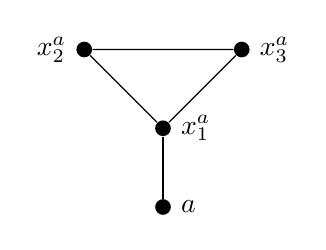
\begin{tikzpicture}
\tikzstyle{vertex}=[circle,fill=black,minimum size=1pt,inner sep=2pt]
\node[vertex,label=left:$x_2^a$] (2) at (0,0) {};
\node[vertex,label=right:$x^a_3$] (3) at (2,0) {};
\node[vertex,label=right:$x^a_1$] (1) at (1,-1) {};
\node[vertex,label=right:$a$] (a) at (1,-2) {};
\draw (2) -- (3) -- (1) -- (2);
\draw (a) -- (1);
\end{tikzpicture}
\end{center}

If \(a<b\), then \(G_A\) will have vertices \(y_1^{a,b},y_2^{a,b},y_3^{a,b}\) and
contain the subgraph

\begin{center}
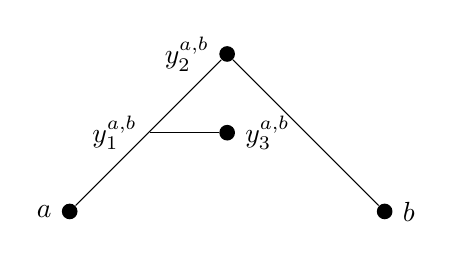
\begin{tikzpicture}
\tikzstyle{vertex}=[circle,fill=black,minimum size=1pt,inner sep=2pt]
\tikzstyle{empty}=[circle,fill=black,minimum size=1pt,inner sep=0]
\node[vertex,label=left:$y_2^{a,b}$] (2) at (2,2) {};
\node[label=left:$y_1^{a,b}$,inner sep=0] (1) at (1,1) {};
\node[vertex,label=right:$y_3^{a,b}$] (3) at (2,1) {};
\node[vertex,label=left:$a$] (a) at (0,0) {};
\node[vertex,label=right:$b$] (b) at (4,0) {};
\draw (a) -- (2);
\draw (1) -- (3);
\draw (2) -- (b);
\end{tikzpicture}
\end{center}


Let \(V_A=A\cup\{x_1^a,x_2^a,x_3^a:a\in
   A\}\cup\{y_1^{a,b},y_2^{a,b},y_3^{a,b}:a,b\in A\text{ and }a<b\}\), and let
\(R_A\) be the smallest symmetric relation containing all edges drawn above.

For example, if \(A\) is the three-element linear order \(a<b<c\), then \(G_A\) is
the graph

\begin{center}
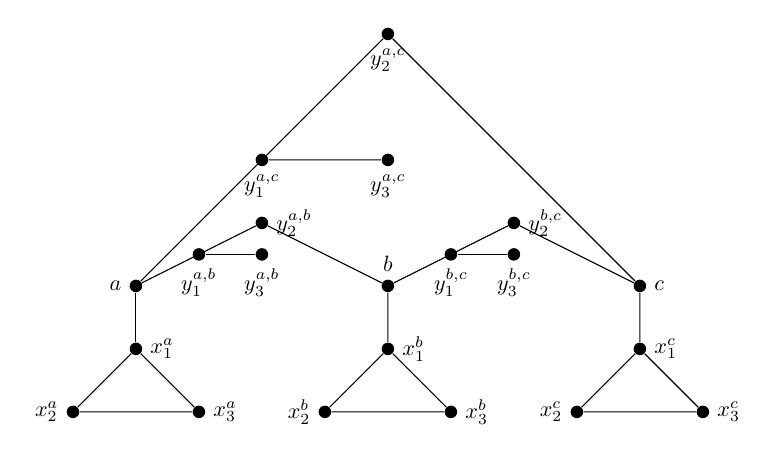
\begin{tikzpicture}[scale=0.8,transform shape]
\tikzstyle{vertex}=[circle,fill=black,minimum size=1pt,inner sep=2pt]
\tikzstyle{empty}=[circle,fill=black,minimum size=1pt,inner sep=0]
\node[vertex,label=left:$x_2^a$] (a2) at (0,0) {};
\node[vertex,label=left:$x_2^b$] (b2) at (4,0) {};
\node[vertex,label=left:$x_2^c$] (c2) at (8,0) {};
\node[vertex,label=right:$x_1^c$] (c1) at (9,1) {};
\node[vertex,label=right:$x_1^b$] (b1) at (5,1) {};
\node[vertex,label=right:$x_1^a$] (a1) at (1,1) {};
\node[vertex,label=right:$x_3^a$] (a3) at (2,0) {};
\node[vertex,label=right:$x_3^b$] (b3) at (6,0) {};
\node[vertex,label=right:$x_3^c$] (c3) at (10,0) {};
\node[vertex,label=left:$a$] (a) at (1,2) {};
\node[vertex,label=above:$b$] (b) at (5,2) {};
\node[vertex,label=right:$c$] (c) at (9,2) {};
\node[vertex,label=below:$y_1^{a,b}$] (ab1) at (2,2.5) {};
\node[vertex,label=below:$y_1^{b,c}$] (bc1) at (6,2.5) {};
\node[vertex,label=below:$y_3^{a,b}$] (ab3) at (3,2.5) {};
\node[vertex,label=right:$y_2^{a,b}$] (ab2) at (3,3) {};
\node[vertex,label=below:$y_3^{b,c}$] (bc3) at (7,2.5) {};
\node[vertex,label=right:$y_2^{b,c}$] (bc2) at (7,3) {};
\node[vertex,label=below:$y_3^{a,c}$] (ac3) at (5,4) {};
\node[vertex,label=below:$y_2^{a,c}$] (ac2) at (5,6) {};
\node[vertex,label=below:$y_1^{a,c}$] (ac1) at (3,4) {};
\draw (a2) -- (a1) -- (a3) -- (a2);
\draw (a1) -- (a);
\draw (b2) -- (b1) -- (b3) -- (b2);
\draw (b1) -- (b);
\draw (c2) -- (c1) -- (c3) -- (c2);
\draw (c1) -- (c);
\draw (a) -- (ac2);
\draw (ac2) -- (c);
\draw (a) -- (ab2);
\draw (ab1) -- (ab3);
\draw (ac1) -- (ac3);
\draw (bc1) -- (bc3);
\draw (b) -- (bc2);
\draw (b) -- (ab2);
\draw (c) -- (bc2);
\end{tikzpicture}
\end{center}

Let \(\call=\{R\}\) where \(R\) is a binary relation. Let \(\phi(x,u,v,w)\) be the
formula asserting that \(x,u,v,w\) are distinct, there are edges
\((x,u),(u,v),(v,w),(u,w)\) and these are the only edges involving \(u,v,w\).
\(G_A\models\phi(a,x_1^a,x_2^a,x_3^a)\) for all \(a\in A\).

\(\psi(x,y,u,v,w)\) asserts that \(x,y,u,v,w\) are distinct. \((x,u),(u,v),(u,w),(v,y)\)

Define \(\theta_i(z)\) as follows:
\begin{align*}
&\theta_0(z):=\exists u\exists v\exists w\;\phi(z,u,v,w)\\
&\theta_1(z):=\exists x\exists v\exists w\;\phi(x,z,v,w)\\
&\theta_2(z):=\exists u\exists u\exists w\;\phi(x,u,z,w)\\
&\theta_3(z):=\exists x\exists y\exists v\exists w\;\psi(x,y,z,v,w)\\
&\theta_4(z):=\exists x\exists y\exists u\exists w\;\psi(x,y,u,z,w)\\
&\theta_5(z):=\exists x\exists y\exists u\exists v\;\psi(x,y,u,v,z)\\
\end{align*}
If \(a,b\in A\) and \(a<b\), then
\begin{equation*}
G_A\models\theta_0(a)\wedge\theta_1(x^a_1)\wedge\theta_2(x^a_2)\wedge
\theta_2(x^a_3)
\end{equation*}
and 
\begin{equation*}
G_A\models\theta_3(y_1^{a,b})\wedge\theta_4(y_2^{a,b})\wedge\theta_5(
y_3^{a,b})
\end{equation*}
\begin{lemma}[]
If \((A,<)\) is a linear order, then for all vertices \(x\) in \(G\), there is a
unique \(i\le 5\) s.t. \(G_A\models\theta_i(x)\)
\end{lemma}

Let \(T\) be the \(\call\)-theory with the following axioms
\begin{enumerate}
\item \(R\) is symmetric and irreflexive
\item for all \(x\), exactly one \(\theta_i\) holds
\item if \(\theta_0(x)\) and \(\theta_0(y)\) then \(\neg R(x,y)\)
\item if \(\exists u\exists v\exists w\;\psi(x,y,u,v,w)\\\) then
\(\forall u_1\forall v_1\forall w_1\neg\psi(y,x,u_1,v_1,w_1)\)
\item if \(\exists u\exists v\exists w\;\psi(x,y,u,v,w)\) and 
\(\exists u\exists v\exists w\;\psi(y,z,u,v,w)\) then\par
\(\exists u\exists v\exists w\;\psi(x,z,u,v,w)\)
\item if \(\theta_0(x)\) and \(\theta_0(y)\), then either \(x=y\) or 
\(\exists u\exists v\exists w\;\psi(x,y,u,v,w)\) or
\(\exists u\exists v\exists w\;\psi(y,x,u,v,w)\)
\item if \(\phi(x,u,v,w)\wedge\phi(x,u',v',w')\), then
\(u=u',v=v',w=w'\)
\item if \(\psi(x,y,u,v,w)\wedge\psi(x,y,u',v',w')\), then
\(u'=u,v=v',w=w'\)
\end{enumerate}


If \((A,<)\) is a linear order, then \(G_A\models T\)

Suppose \(G\models T\). Let \(X_G=\{x\in G:G\models\theta_0(x)\}\)

\begin{lemma}[]
If \((A,<)\) is a linear order, then \((X_{G_A},<_{G_A})\cong(A,<)\). Moreover,
\(G_{X_G}\cong G\) for all \(G\models T\)
\end{lemma}

\begin{definition}[]
An \(\call_0\)-structure \(\caln\) is \textbf{interpretable} in an
\(\call\)-structure \(M\) if there is a definable \(X\subseteq M^n\), a definable
equivalence relation \(E\) on \(X\), and for each symbol of \(\call_0\) we can find
definable \(E\)-invariant sets on X s.t. \(X/E\) with the induced structure is
isomorphic to \(\caln\)
\end{definition}
\subsection{Answers to Exercises}
\label{sec:org76016f9}
\begin{exercise}
\begin{enumerate}
\item transform \(\psi\) to CNF
\item prenex normal form
\end{enumerate}
\end{exercise}
\begin{exercise}
\begin{enumerate}
\item 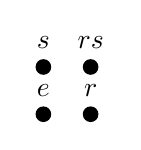
\begin{tikzpicture}[scale=0.6]
\tikzstyle{vertex}=[circle,fill=black,minimum size=1pt,inner sep=2pt]
\node[vertex,label=above:$s$] (1) at (0,1) {};
\node[vertex,label=above:$e$] (0) at (0,0) {};
\node[vertex,label=above:$r$] (2) at (1,0) {};
\node[vertex,label=above:$rs$] (3) at (1,1) {};
\end{tikzpicture}
\item enumerate \(\calm\)'s functions, relations and constants
\end{enumerate}
\end{exercise}
\begin{exercise}
\footnote{\href{https://math.stackexchange.com/questions/1170953/let-alpha-be-any-cardinal-there-are-at-most-2-alpha-cup-mathscrl}{stackexchange}}
Note that every \(\call\)-structure \(\calm\) of size \(\kappa\) is isomorphic to an
\(\call\)-structure with domain \(\kappa\). For each relation symbols, we have \(2^\kappa\)
options. If the language has size \(\lambda\), this is at most 
\((2^\kappa)^\lambda=2^{\kappa\cdot\lambda}=2^{\max(\lambda,\kappa)}\)
\end{exercise}

\begin{exercise}
\begin{align*}
T\models\phi&\Leftrightarrow\forall \calm\;\calm\models T\to\calm\models\phi\\
&\Leftrightarrow\forall \calm\;\calm\models T'\to\calm\models\phi\\
&\Leftrightarrow T'\models\phi
\end{align*}
\end{exercise}
\begin{exercise}
Follow the definition
\end{exercise}

\begin{exercise}
Since there is no model \(\calm\) s.t. \(\calm\models T\). It's true that 
\(T\models \phi\)
\end{exercise}

\begin{exercise}
\begin{enumerate}
\item Suppose \(\calm\models\phi\), then \(E^\calm\) is an equivalent relation and
each equivalence class's cardinality is 2
\item follows from number theory
\item \cite{DBLP:journals/bsl/DurandJMM12}
\end{enumerate}
\end{exercise}

\begin{exercise}
TBD
\end{exercise}

\begin{exercise}
\(G(f)=\{(\bar{x},\bar{y})\in M^{n+m}\mid\phi(\bar{x},\bar{y})\}\) and 
\(G(g)=\{(\bar{y},\bar{z})\in M^{m+l}\mid\psi(\bar{y},\bar{z})\}\). Hence
\(G(g\circ f)=\{(\bar{x},\bar{z})\in M^{n+l}\mid \phi(\bar{x},\bar{y})
   \wedge \psi(\bar{y},\bar{z})\}\)
\end{exercise}

\begin{exercise}
\(\phi(\bar{a},b)\) really defines a function and since 
\(\phi(\bar{a},y)\to y=b\)
\end{exercise}

\section{Basic Techniques}
\label{sec:org2bfff3a}
\subsection{The Compactness Theorem}
\label{sec:org1fe8005}

Some points of proofs
\begin{itemize}
\item Proofs are finite
\item (Soundness) If \(T\vdash\phi\), then \(T\models\phi\)
\item If \(T\) is a finite set of sentences, then there is an algorithm that,
when given a sequence of \(\call\)-formulas \(\sigma\) and an \(\call\)-sentence \(\phi\),
will decide whether \(\sigma\) is a proof of \(\phi\) from \(T\)
\end{itemize}

\index{recursive}
A language \(\call\) is \textbf{recursive} if there is an algorithm that decides
whether a sequence of symbols is an \(\call\)-formula. An \(\call\)-theory
\(T\) is \textbf{recursive} if there is an algorithm that when given an
\(\call\)-sentence \(\phi\) as input, decides whether \(\phi\in T\)

\begin{proposition}[]
\label{prop2.1.1}
If \(\call\) is a recursive language and \(T\) is a recursive \(\call\)-theory,
then \(\{\phi:T\vdash\phi\}\) is recursively enumerable; that is, there is an
algorithm that when given \(\phi\) as input will halt accepting if \(T\vdash\phi\)
and not halt if \(T\not\vdash\phi\)
\end{proposition}
\begin{proof}
There is \(\sigma_0,\sigma_1,\dots\) a computable listing of all finite
sequence of \(\call\)-formulas. At stage \(i\), we check to see whether
\(\sigma_i\) is a proof of \(\psi\) from \(T\). If it is, then halt.
\end{proof}

\begin{theorem}[Gödel's Completeness Theorem]
Let \(T\) be an \(\call\)-theory and \(\phi\) an \(\call\)-sentence, then
\(T\models\phi\) if and only if \(T\vdash \phi\)
\end{theorem}

We say that an \(\call\)-theory \(T\) is \textbf{inconsistent} if
\(T\vdash(\phi\wedge\neg\phi)\) for some sentence \(\phi\).

\begin{corollary}[]
\(T\) is consistent if and only if \(T\) is satisfiable
\end{corollary}

\begin{proof}
Supose that \(T\) is not satisfiable, then every model of \(T\) is a model of
\(\phi\wedge\neg\phi\). Thus by the Completeness theorem
\(T\vdash(\phi\wedge\neg\phi)\) 
\end{proof}


\begin{theorem}[Compactness Theorem]
\(T\) is satisfiable if and only if every finite subset of \(T\) is satisfiable
\end{theorem}

\begin{proof}
If \(T\) is not satisfiable, then \(T\) is inconsistent. Let \(\sigma\) be a proof of
a contradiction from  \(T\). Because \(\sigma\) is finite, only finitely many
assumptions from \(T\) are used in the proof. Thus there is a finite
\(T_0\subseteq T\) s.t. \(\sigma\) is a proof of a contradiction from \(T_0\)
\end{proof}

\subsubsection{Henkin Constructions}
\label{sec:orgef35ab6}
\index{finitely satisfiable}
A theory \(T\) is \textbf{finitely satisfiable} if every finite subset of \(T\) is
satisfiable. We will show that every finitely satisfiable theory \(T\) is
satisfiable.

\begin{definition}[]
We say that an \(\call\)-theory \(T\) has the \textbf{witness property} if whenever
\(\phi(v)\) is an \(\call\)-formula with one free variable \(v\), then there is
a constant symbol \(c\in\call\) s.t. \(T\vdash(\exists v\phi(v))\to\phi(c)\in T\)

An \(\call\)-theory \(T\) is \textbf{maximal} if for all \(\phi\) either \(\phi\in T\) or
\(\neg\phi\in T\)
\end{definition}

\begin{lemma}[]
\label{lemma2.1.6}
Suppose \(T\) is a maximal and finitely satisfiable \(\call\)-theory. If
\(\Delta\subseteq T\) is finite and \(\Delta\models\psi\), then \(\psi\in T\)
\end{lemma}

\begin{proof}
If \(\psi\not\in T\), then \(\neg\psi\in T\) but \(\Delta\cup\{\psi\}\) is
unsatisfiable 
\end{proof}

\begin{lemma}[]
\label{lemma2.1.7}
Suppose that \(T\) is a maximal and finitely satisfiable \(\call\)-theory with
the witness property. Then \(T\) has a model. In fact, if \(\kappa\) is a cardinal
and \(\call\) has at most \(\kappa\) constant symbols, then there is
\(\calm\models T\) with \(\abs{\calm}\le\kappa\)
\end{lemma}

\begin{proof}
Let \(\calc\) be the set of constant symbols of \(\call\). For \(c,d\in\calc\),
we say \(c\sim d\) if \(c=d\in T\)

\textbf{Claim 1} \(\sim\) is an equivalence relation. 

The universe of our model will be \(M=\calc/\sim\). Clearly
\(\abs{M}\le\kappa\). We let \(c^*\) denote the equivalence class of \(c\) and
interprete \(c\) as its equivalence class, that is, \(c^\calm=c^*\)

Suppose that \(R\) is an \(n\)-ary relation symbol of \(\call\)

\textbf{Claim 2} Suppose that \(c_1,\dots,c_n,d_1,\dots,d_n\in\calc\) and \(c_i\sim d_i\)
for \(i=1,\dots,n\), then \(R(\bar{c})\) if and only if \(R(\bar{d})\)

By Lemma \ref{lemma2.1.6}, if one of \(R(\bar{c})\) and \(R(\bar{d})\) is
in \(T\), then both are in \(T\)


\begin{equation*}
R^\calm=\{(c_1^*,\dots,c_n^*):R(c_1,\dots,c_n)\in T\}
\end{equation*}
Suppose that \(f\) is an \(n\)-ary function symbol of \(\call\) and
\(c_1,\dots,c_n\in\calc\). Because  \(\underline{\emptyset\models\exists
    vf(c_1,\dots,c_n)=v}\), and \(T\) has the witness property, then there is
\(c_{n+1}\in\calc\) s.t. \(f(c_1,\dots,c_n)=c_{n+1}\in T\). As above, if
\(d_i\sim c_i\) for \(i=1,\dots,n+1\), then \(f(d_1,\dots,d_n)=d_{n+1}\in T\).
Thus we get a well-defined function \(f^\calm:M^n\to M\) by
\begin{equation*}
f^\calm(c_1^*,\dots,c_n^*)=d^*\text{ if and only if }f(c_1,\dots,c_n)=d\in T
\end{equation*}

\textbf{Claim 3} Suppose that \(t\) is a term using free variables from
\(v_1,\dots,v_n\). If \(c_1,\dots,c_n,d\in\calc\), then \(t(c_1,\dots,c_n)=d\in
    T\) if and only if \(t^\calm(c_1^*,\dots,c_n^*)=d^*\)

(\(\Rightarrow\)) If \(t\) is a constant symbol, then \(c=d\in T\) and
\(c^\calm=c^*=d^*\)

If \(t\) is the variable \(v_i\), then \(c_i=d\in T\) and 
\(t^\calm(c_1^*,\dots,c_n^*)=c_i^*=d^*\)

Suppose that the claim is true for \(t_1,\dots,t_m\) and \(t\) is
\(f(t_1,\dots,t_m)\). Using the witness property and Lemma \ref{lemma2.1.6},
we can find \(d,d_1,\dots,d_n\in\calc\) s.t. \(t_i(c_1,\dots,c_n)=d_i\in T\)
for \(i\le m\) and \(f(d_1,\dots,d_m)=d\in T\). By our induction hypothesis, 
\(t_i^\calm(c_1^*,\dots,c_n^*)=d_i^*\) and
\(f^\calm(d_1^*,\dots,d_m^*)=d^*\). Thus \(t^\calm(c_1^*,\dots,c_n^*)=d^*\)

(\(\Leftarrow\)) Suppose \(t^\calm(c_1^*,\dots,c_n^*)=d^*\). By the witness
property, there is a \(e\in\calc\) s.t. \(t(c_1,\dots,c_n)=e\in T\). Using the
\((\Rightarrow)\) direction of the proof, \(t^\calm(c_1^*,\dots,c_n^*)=e^*\).
Thus \(e^*=d^*\) and \(e=d\in T\)


\textbf{Claim 4} For all \(\call\)-formulas \(\phi(v_1,\dots,v_n)\) and
\(c_1,\dots,c_n\in\calc\), \(\calm\models\phi(\bar{c}^*)\) if and only if
\(\phi(\bar{c})\in T\)

Suppose that \(\phi\) is \(t_1=t_2\). By Lemma \ref{lemma2.1.6} and the
witness property, we can find \(d_1\) and \(d_2\) s.t. 
\(t_1(\bar{c})=d_1,t_2(\bar{c})=d_2\in T\). By Claim 3,
\(t_i^\calm(\bar{c}^*)=d_i^*\). Then
\begin{align*}
\calm\models\phi(\bar{c}^*)&\Leftrightarrow d_1^*=d_2^*\\
&\Leftrightarrow d_1=d_2\in T\\
&\Leftrightarrow t_1(\bar{c})=t_2(\bar{c})\in T
\end{align*}

Suppose that \(\phi\) is \(R(t_1,\dots,t_m)\). There are \(d_1,\dots,d_m\in\calc\)
s.t. \(t_i(\bar{c})=d_i\in T\). Thus
\begin{align*}
\calm\models\phi(\bar{c}^*)&\Leftrightarrow \bar{d}^*\in R^\calm\\
&\Leftrightarrow R(\bar{d})\in T\\
&\Leftrightarrow\phi(\bar{c})\in T
\end{align*}

Suppose that the claim is true for \(\phi\). If
\(\calm\models\neg\phi(\bar{c}^*)\), then
\(\calm\not\models\phi(\bar{c}^*)\). By the inductive hypothesis,
\(\phi(\bar{c})\not\in T\). Thus by maximality, \(\neg\phi(\bar{c})\in T\). On
the other hand, if \(\neg\phi(\bar{c})\in T\), then because \(T\) is finitely
satisfiable, \(\phi(\bar{c})\not\in T\). Thus, by induction,
\(\calm\not\models\phi(\bar{c}^*)\).
\end{proof}

\begin{lemma}[]
\label{lemma2.1.8}
Let \(T\) be a finitely satisfiable \(\call\)-theory. There is a language
\(\call^*\supseteq\call\) and \(T^*\supseteq T\) a finitely satisfiable
\(\call^*\)-theory s.t. any \(\call^*\)-theory extending \(T^*\) has the
witness property. We can choose \(\call^*\) s.t.
\(\abs{\call^*}=\abs{\call}+\aleph_0\) 
\end{lemma}

\begin{proof}
We first show that there is a language \(\call_1\supseteq\call\) and a
finitely satisfiable \(\call_1\)-theory \(\call_1\supseteq T\) s.t. for any
\(\call\)-formula \(\phi(v)\) there is an \(\call_1\)-constant symbol \(c\) s.t.
\(T_1\models(\exists v\phi(v))\to\phi(c)\). For each \(\call\)-formula
\(\phi(v)\), let \(c_\phi\) be a new constant symbol and let
\(\call_1=\call\cup\{c_\phi:\phi(v)\text{ an }\call\text{-formula}\}\). For
each \(\call\)-formula \(\phi(v)\), let \(\Theta_\phi\) be the
\(\call_1\)-sentence
\((\exists v\phi(v))\to\phi(c_\phi)\). Let
\(T_1=T\cup\{\Theta_\phi:\phi(v)\text{ an }\call\text{-formula}\}\)

\textbf{Claim} \(T_1\) is finitely satisfiable

Suppose that \(\Delta\) is a finite subset of \(T_1\). Then
\(\Delta=\Delta_0\cup\{\Theta_{\phi_1},\dots, \Theta_{\phi_n}\}\) where
\(\Delta_0\) is a finite subset of \(T\) and there is \(\calm\models\Delta_0\). We
will make \(\calm\) into an
\(\call\cup\{c_{\phi_1},\dots,c_{\phi_n}\}\)-structure \(\calm'\). If
\(\calm\models\exists v\phi(v)\), choose \(a_i\) some element of \(M\) s.t.
\(\calm\models\phi(a_i)\) and let \(c_{\phi_i}^{\calm'}=a_i\). Otherwise, let
\(c_{\phi_i}^{\calm'}\) be any element of \(\calm\). Clearly
\(\calm'\models\Theta_{\phi_i}\) for \(i\le n\). Thus \(T_1\) is finitely
satisfiable.

We now iterate the construction above to build a sequence of languages
\(\call\subseteq\call_1\subseteq\call_2\subseteq\dots\) and a sequence of
finitely satisfiable \(\call_i\)-theories \(T\subseteq T_1\subseteq
    T_2\subseteq\dots\) s.t. if \(\phi(v)\) is an \(\call_i\)-formula then there is
a constant symbol \(c\in\call_{i+1}\) s.t. \(T_{i+1}\models(\exists
    v\phi(v))\to\phi(c)\)

Let \(\call^*=\bigcup\call_i\) and \(T^*=\bigcup T_i\). 
If \(\abs{\call_i}\) is the number of relation, function and constant
symbols in \(\call_i\), then there are at most \(\abs{\call_i}+\aleph_0\)
formulas in \(\call_i\).
Thus by induction,
\(\abs{\call^*}=\abs{\call}+\aleph_0\) 
\end{proof}

\begin{lemma}[]
\label{2.1.9}
Suppose that \(T\) is a finitely satisfiable \(\call\)-theory and \(\phi\) is an
\(\call\)-sentence, then either \(T\cup\{\phi\}\) or \(T\cup\{\neg\phi\}\) is
finitely satisfiable
\end{lemma}

\begin{corollary}[]
\label{cor2.1.10}
If \(T\) is a finitely satisfiable \(\call\)-theory, then there is a maximal
finitely satisfiable \(\call\)-theory \(T'\supseteq T\)
\end{corollary}
\begin{proof}
Let \(I\) be the set of all finitely satisfiable \(\call\)-theory containing
\(T\). We partially order \(I\) by inclusion. If \(C\subseteq I\) is a chain, let
\(T_C=\bigcup\{\Sigma:\Sigma\in C\}\). If \(\Delta\) is a finite subset of
\(T_C\), then there is a \(\Sigma\in C\) s.t. \(\Delta\subseteq\Sigma\), so \(T_C\)
is finitely satisfiable and \(T_C\supseteq\Sigma\) for all \(\Sigma\in C\). Thus
every chain in \(I\) has an upper bound, and we can apply Zorn's lemma to find
a \(T'\in I\) maximal w.r.t. the partial order.
\end{proof}


\begin{theorem}[strengthening of Compactness Theorem]
\label{thm2.1.11}
If \(T\) is a finitely satisfiable \(\call\)-theory and \(\kappa\) is an infinite
cardinal with \(\kappa\ge\abs{\call}\), then there is a model of \(T\) of
cardinality at most \(\kappa\)
\end{theorem}

\begin{proof}
By Lemma \ref{lemma2.1.8}, we can find \(\call^*\supseteq\call\) and 
\(T^*\supseteq T\) a finitely satisfiable \(\call^*\)-theory s.t. any
\(\call^*\)-theory extending \(T^*\) has the witness property and the
cardinality of \(\call^*\) is at most \(\kappa\). By Corollary \ref{cor2.1.10}, we can
find a maximal finitely satisfiable \(\call^*\)-theory 
\(T'\supseteq T^*\). Because \(T'\) has the witness property, Lemma
\ref{lemma2.1.7} ensures that there is \(\calm\models T\) with \(\abs{M}\le\kappa\)
\end{proof}

\begin{proposition}[]
Let \(\call=\{\cdot,+,<,0,1\}\) and let \(\Th(\N)\) be the full \(\call\)-theory
of the natural numbers. There is \(\calm\models\Th(\N)\) and \(a\in M\) s.t. \(a\)
is larger than every natural number
\end{proposition}

\begin{proof}
Let \(\call^*=\call\cup\{c\}\) where \(c\) is a new constant symbol and let
\begin{equation*}
T=\Th(\N)\cup\{\underbrace{1+1+\dots+1}_{n\text{-times}}<c:\text{for }n=1,2,\dots\} 
\end{equation*}
If \(\Delta\) is a finite subset of \(T\) we can make \(\N\) a model of \(\Delta\) by
interpreting \(c\) as a suitably large natural number. Thus \(T\) is finitely
satisfiable and there is \(\calm\models T\).
\end{proof}
\begin{lemma}[]
\label{lemma2.1.14}
If \(T\models\phi\), then \(\Delta\models T\) for some finite \(\Delta\subseteq T\)
\end{lemma}
\begin{proof}
Suppose not. Let \(\Delta\subseteq T\) be finite. Because
\(\Delta\not\models\phi\), \(\Delta\cup\{\neg\phi\}\) is satisfiable. Thus
\(T\cup\{\neg\phi\}\) is finitely satisfiable and by the compactness theorem,
\(T\not\models\phi\) 
\end{proof}



\subsection{Complete Theories}
\label{sec:org02b5902}
\index{complete}
\begin{definition}[]
An \(\call\)-theory \(T\) is called \textbf{complete} if for any \(\call\)-sentence \(\phi\)
either \(T\models\phi\) or \(T\models\neg\phi\)
\end{definition}

For \(\calm\) an \(\call\)-structure, then the full theory
\begin{equation*}
\Th(\calm)=\{\phi:\phi\text{ is an }\call\text{-sentence and }
\calm\models\phi\}
\end{equation*}
is a complete theory.

\begin{proposition}[]
\label{prop2.2.2}
Let \(T\) be an \(\call\)-theory with infinite models. If \(\kappa\) is an infinite
cardinal and \(\kappa\ge\abs{\call}\), then there is a model of \(T\) of
cardinality \(\kappa\)
\end{proposition}

\begin{proof}
Let \(\call^*=\call\cup\{c_\alpha:\alpha<\kappa\}\), where each \(c_\alpha\) is
new constant symbol, and let \(T^*\) be the \(\call^*\)-theory
\(T\cup\{c_\alpha\neq c_\beta:\alpha,\beta<\kappa,\alpha\neq\beta\}\). Clearly
if \(\calm\models T^*\), then \(\calm\) is a model of \(T\) of cardinality at least
\(\kappa\).
Thus by Theorem \ref{thm2.1.11}, it suffices to show that \(T^*\) is finitely
satisfiable. But if \(\Delta\subseteq T^*\) is finite, then \(\Delta\subseteq
   T\cup\{c_\alpha\neq c_\beta:\alpha\neq\beta,\alpha,\beta\in I\}\), where \(I\)
is a finite subset of \(\kappa\). Let \(\calm\) be an infinite model of \(T\). We can
interpret the symbols \(\{c_\alpha:\alpha\in I\}\) as \(\abs{I}\) distinct
elements of \(M\). Because \(\calm\models\Delta\), \(T^*\) is finitely satisfiable.
\end{proof}

\begin{definition}[]
Let \(\kappa\) be an infinite cardinal and let \(T\) be a theory with models of
size \(\kappa\). We say that \(T\) is \textbf{\(\kappa\)-categorical} if any two models of
\(T\) of cardinality \(\kappa\) are isomorphic.
\end{definition}

Let \(\call=\{+,0\}\) be the language of additive groups and let \(T\) be the
\(\call\)-theory of torsion-free divisible Abelian groups. The axioms of \(T\)
are the axioms for Abelian groups together with the axioms
\begin{gather*}
\forall x(x\neq 0\to\underbrace{x+\dots+x}_{n\text{-times}}\neq 0)\\
\forall y\exists x\underbrace{x+\dots+x}_{n\text{-times}}=y
\end{gather*}
for \(n=1,2,\dots\)


\begin{proposition}[]
The theory of torsion-free divisible Abelian groups is \(\kappa\)-categorical for
all \(\kappa>\aleph_0\)
\end{proposition}

\begin{proof}
We first argue that models of \(T\) are essentially vector spaces over the
field of rational numbers \(\Q\). If \(V\) is any vector space over \(\Q\), then
the underlying additive group \(V\) is a model of \(T\). 
Check \href{https://math.stackexchange.com/questions/1550900/necessary-and-sufficient-conditions-for-an-abelian-group-to-be-a-vector-space-ov/1550954}{StackExchange}.
On the other hand, if
\(G\models T\), \(g\in G\) and \(n\in\N\) with \(g>0\), we can find 
\(h\in G\) s.t. \(nh=g\). If \(nk=g\), then \(n(h-k)=0\). Because \(G\) is
torsion-free there is a unique \(h\in G\) s.t. \(nh=g\). We call this element 
\(g/n\). We can view \(G\) as a \(\Q\)-vector space under the action
\(\frac{m}{n}g=m(g/n)\)

Two \(\Q\)-vector spaces are isomorphic if and only if they have the same
dimension. Thus the model of \(T\) are determined up to isomorphism by their
dimension. If \(G\) has dimension \(\lambda\), then \(\abs{G}=\lambda+\aleph_0\). If \(\kappa\)
is uncountable and \(G\) has cardinality \(\kappa\), then \(G\) has dimension \(\kappa\). Thus for
\(\kappa>\aleph_0\) any two models of \(T\) of cardinality \(\kappa\) are isomorphic
\end{proof}

\begin{lemma}[]
\label{lemmamy1}
Field of uncountable cardinality \(\kappa\) has transcendence degree \(\kappa\)
\footnote{\href{https://proofwiki.org/wiki/Field\_of\_Uncountable\_Cardinality\_K\_has\_Transcendence\_Degree\_K}{proofwiki}}
\end{lemma}

\begin{proof}
We prove the theorem for fields with characteristic \(p=0\). 

Since each characteristic 0 field contains a copy of \(\Q\) as its prime
field, we can view \(F\) as a field extension over \(\Q\). We will show that
\(F\) has a subset of cardinality \(\kappa\) which is algebraically independent over
\(\Q\).

We build the claimed subset of \(F\) by transfinite induction and implicit use
of the axiom of choice.

Let \(S_0=\emptyset\)

Let \(S_1\) be a singleton containing some element of \(F\) which is not
algebraic over \(\Q\). This is possible since algebraic numbers are countable

Define \(S_{\alpha+1}\) to be \(S_\alpha\) together with an element of \(F\)
which is not a root of any non-trivial polynomial with coefficients in 
\(\Q\cup S_\alpha\) since there are only 
\(\abs{\Q\cup S_\alpha}=\aleph_0+\abs{\alpha}<\kappa\) polynomials

Define \(S_\beta=\displaystyle\bigcup_{\alpha<\beta}S_\alpha\)

Let \(P(x_1,\dots,x_n)\) be a non-trivial polynomial with coefficients in
\(\Q\) and elements \(a_1,\dots,a_n\) in \(F\). W.L.O.G., it is assumed that
\(a_n\) was added at an ordinal \(\alpha+1\) later than the other elements.
Then \(P(a_1,\dots,a_{n-1},x_n)\) is a polynomial with coefficients in 
\(\Q\cup S_\alpha\). Hence \(P(a_1,\dots,a_n)\neq0\).
\end{proof}

\begin{proposition}[]
\label{prop2.2.5}
\(\ACF_p\) is \(\kappa\)-categorical for all uncountable cardinals \(\kappa\)
\end{proposition}

\begin{proof}
Two algebraically closed fields are isomorphic if and only if they have the
same characteristic and transcendence degree. See
\url{AdvancedModernAlgebra.org}. By Lemma
\ref{lemmamy1}, an algebraically closed field of transcendence degree \(\lambda\) has
cardinality \(\lambda+\aleph_0\).
\end{proof}

\begin{theorem}[Vaught's Test]
\label{thm2.2.6}
Let \(T\) be a satisfiable theory with no finite models that is
\(\kappa\)-categorical for some infinite cardinal \(\kappa\ge\abs{\call}\). Then
\(T\) is complete
\end{theorem}

\begin{proof}
Suppose \(T\) is not complete. Then there is a sentence \(\phi\) s.t. 
\(T\not\models\phi\) and \(T\not\models\neg\phi\). Because
\(T\not\models\psi\) if and only if \(T\cup\{\neg\psi\}\) is satisfiable, the
theories \(T_0=T\cup\{\phi\}\) and \(T_1=T\cup\{\neg\phi\}\) are satisfiable.
Because \(T\) has no finite models, both \(T_0\) and \(T_1\) have infinite
models. By Proposition \ref{prop2.2.2} we can find \(\calm_0\) and
\(\calm_1\) of cardinality \(\kappa\) with \(\calm_i\models T_i\). Because \(\calm_0\)
and \(\calm_1\) disagree about \(\phi\), they are not elementarily equivalent, and
hence by Theorem \ref{thm1.1.10}, nonisomorphic. 
\end{proof}

\begin{definition}[]
We say that an \(\call\)-theory \(T\) is \textbf{decidable} if there is an algorithm
that when given an \(\call\)-sentence \(\phi\) as input decides whether \(T\models\phi\)
\end{definition}

\begin{lemma}[]
\label{lemma2.2.8}
Let \(T\) be a recursive complete satisfiable theory in a recursive language
\(\call\). Then \(T\) is decidable
\end{lemma}

\begin{proof}
Because \(T\) is satisfiable \(A=\{\phi:T\models\phi\}\) and
\(B=\{\phi:T\models\neg\phi\}\) are disjoint. Because \(T\) is consistent 
\(A\cup B\) is the set of all \(\call\)-sentences. By the Completeness
Theorem, \(A=\{\phi:T\vdash\phi\}\) and \(B=\{\phi:T\vdash\neg\phi\}\). By
Proposition \ref{prop2.1.1} \(A\) and \(B\) are recursively enumerable. But any
recursively enumerable set with a recursively enumerable complement is
recursive. 
\end{proof}

\begin{corollary}[]
For \(p=0\) or \(p\) prime, \(ACF_p\) is decidable. In particular, \(\Th(\C)\),
the first-order theory  of the field of complex numbers, is decidable
\end{corollary}

\begin{corollary}[]
Let \(\phi\) be a sentence in the language of rings. The following are equivalent
\begin{enumerate}
\item \(\phi\) is true in the complex number
\item \(\phi\) is true in every algebraically closed field of characteristic zero
\item \(\phi\) is true in some algebraically closed field of characteristic zero
\item There are arbitrarily large primes \(p\) s.t. \(\phi\) is true in some
algebraically closed field of characteristic \(p\)
\item There is an \(m\) s.t. for all \(p>m\), \(\phi\) is true in all algebraically
closed fields of characteristic \(p\)
\end{enumerate}
\end{corollary}

\begin{proof}
By Proposition \ref{prop2.2.5} and Vaught's Test, \(\ACF_p\) is complete.

\((2)\to(5)\). Suppose that \(\ACF_0\models\phi\). By Lemma \ref{lemma2.1.14},
there is a finite \(\Delta\subseteq\ACF_0\) s.t. \(\Delta\models\phi\). Thus
if we choose \(p\) large enough, then \(\ACF_p\models\Delta\).

\((4)\to(2)\). Suppose \(\ACF_0\not\models\phi\). Because \(\ACF_0\) is
complete, \(\ACF_0\models\neg\phi\).
\end{proof}

\subsection{Up and Down}
\label{sec:org141e510}


\begin{definition}[]
If \(\calm\) and \(\caln\) are \(\call\)-structures, then an
\(\call\)-embedding \(j:\calm\to\caln\) is called an \textbf{elementary embedding} if
\begin{equation*}
\calm\models\phi(a_1,\dots,a_n)\leftrightarrow\caln\models\phi(j(a_1),\dots,j(a_n))
\end{equation*}
for all \(\call\)-formulas \(\phi(v_1,\dots,v_n)\) and all \(a_1,\dots,a_n\in
   M\)

If \(\calm\) is a substructure of \(\caln\), we say that it is an \textbf{elementary
substructure} and write \(\calm\prec\caln\) if the inclusion map is elementary.
\(\caln\) is an \textbf{elementary extension} of \(\calm\)
\end{definition}

\begin{definition}[]
\(\calm\) is an \(\call\)-structure. Let \(\call_M\) be the language where we
add to \(\call\) constant symbols \(m\) for each element of \(M\). The \textbf{atomic
diagram} of \(\calm\) is \(\{\phi(m_1,\dots,m_n):\phi\text{ is either an atomic
   }\call\text{-formula or the negation of an atomic }\call\text{-formula and
   }\calm\models\phi(m_1,\dots.m_n)\}\).
The \textbf{elementary diagram} of \(\calm\) is 
\begin{equation*}
\{\phi(m_1,\dots,m_n):\calm\models\phi(m_1,\dots,m_n),\phi\text{ an 
\(\call\)-formula}\}
\end{equation*}

We let \(\Diag(\calm)\) and \(\Diag_{\el}(\calm)\) denote the atomic and
elementary diagrams of \(\calm\)
\end{definition}

\begin{lemma}[]
\label{lemma2.3.3}
\begin{enumerate}
\item Suppose that \(\caln\) is an \(\call_M\)-structure and
\(\caln\models\Diag(\calm)\), then viewing \(\caln\) as an
\(\call\)-structure, there is an \(\call\)-embedding of \(\calm\) into \(\caln\)
\item If \(\caln\models\Diag_{\el}(\calm)\), then there is an elementary
embedding of \(\calm\) into \(\caln\)
\end{enumerate}
\end{lemma}

\begin{proof}
\begin{enumerate}
\item Let \(j:M\to N\) by \(j(m)=m^\caln\). If \(m_1\neq m_2\in\Diag(\calm)\);
thus \(j(m_1)\neq j(m_2)\) so \(j\) is an embedding. If \(f\) is a function
symbols of \(\call\) and \(f^\calm(m_1,\dots,m_n)=m_{n+1}\), then
\(f(m_1,\dots,m_n)=m_{n+1}\) is a formula in \(\Diag(\calm)\) and 
\(f^\caln(j(m_1),\dots,j(m_n))=j(m_{n+1})\). If \(R\) is a relation symbol
and \(\bar{m}\in R^\calm\), then \(R(m_1,\dots,m_n)\in\Diag(\calm)\) and 
\((j(m_1),\dots,j(m_{n}))\in R^\caln\). Hence \(j\) is an
\(\call\)-embedding
\item \(j\) is elementary.
\end{enumerate}
\end{proof}

\begin{theorem}[Upward Löwenheim–Skolem Theorem]
Let \(\calm\) be an infinite \(\call\)-structure and \(\kappa\) be an infinite
cardinal \(\kappa\ge\abs{\calm}+\abs{\call}\). Then, there is \(\caln\) an
\(\call\)-structure of cardinality \(\kappa\) and \(j:\calm\to\caln\) is elementary
\end{theorem}

\begin{proof}
Because \(\calm\models\Diag_{\el}(\calm)\), \(\Diag_{\el}(\calm)\) is
satisfiable. By Theorem \ref{thm2.1.11}, there is
\(\caln\models\Diag_{\el}(\calm)\) of cardinality \(\kappa\). By Lemma \ref{lemma2.3.3},
there is an elementary \(j:\calm\to\caln\)
\end{proof}

\begin{proposition}[Tarski-Vaught Test]
\label{prop2.3.5}
Suppose that \(\calm\) is a substructure of \(\caln\). Then \(\calm\) is an
elementary substructure if and only if, for any formula \(\phi(v,\bar{w})\) and 
\(\bar{a}\in M\), if there is \(b\in N\) s.t.
\(\caln\models\phi(b,\bar{a})\), then there is \(c\in M\) s.t.
\(\caln\models\phi(c,\bar{a})\) 
\end{proposition}

\begin{proof}
We need to show that for all \(\bar{a}\in M\) and all \(\call\)-formulas
\(\psi(\bar{v})\)
\begin{equation*}
\calm\models\psi(\bar{a})\Leftrightarrow\caln\models\psi(\bar{a})
\end{equation*}

In Proposition \ref{prop1.1.8}, we showed that if \(\phi(\bar{v})\) is quantifier
free then \(\calm\models\phi(\bar{a})\) if and only if \(\phi(\bar{a})\)
\end{proof}

We say that an \(\call\)-theory \(T\) has \textbf{built-in Skolem functions} if for all
\(\call\)-formulas \(\phi(v,w_1,\dots,w_n)\) there is a function symbol \(f\) s.t.\\
\(T\models\forall\bar{w}((\exists
   v\phi(v,\bar{w}))\to\phi(f(\bar{w}),\bar{w}))\). In other words, there are
enough function symbols in the language to witness all existential statements.

\begin{lemma}[]
\label{lemma2.3.6}
Let \(T\) be an \(\call\)-theory. There are \(\call^*\supseteq\call\) and 
\(T^*\supseteq T\) an \(\call^*\)-theory s.t. \(T^*\) has built-in Skolem
functions, and if \(\calm\models T\), then we can expand \(\calm\) to 
\(\calm^*\models T^*\). We can choose \(\call^*\) s.t.
\(\abs{\call^*}=\abs{\call}+\aleph_0\).

We call \(T^*\) a \textbf{skolemization} of \(T\)
\end{lemma}

\begin{proof}
We build a sequence of languages
\(\call=\call_0\subseteq\call_1\subseteq\dots\) and \(\call_i\)-theories
\(T_i\) s.t. \(T=T_0\subseteq T_1\subseteq\dots\)

Given \(\call_i\), let
\(\call_{i+1}=\call\cup\{f_\phi:\phi(v,w_1,\dots,w_n)\text{ an
   }\call_i\text{-formula},n=1,2,\dots\}\), 
where \(f_\phi\) is an \(n\)-ary function symbol. For \(\phi(v,\bar{w})\) an
\(\call_i\)-formula, let \(\Psi_\phi\) be the sentence
\begin{equation*}
\forall\bar{w}((\exists v\phi(v,\bar{w}))\to\phi(f_\phi(\bar{w}),\bar{w}))
\end{equation*}
and let \(T_{i+1}=T_i\cup\{\Psi_\phi:\phi\text{ an
   }\call_i\text{-formula}\}\)

\textbf{Claim} If \(\calm\models T_i\), then we can interpret the function symbols of
\(\call_{i+1}\backslash\call_i\) so that \(\calm\models T_{i+1}\)

Let \(c\) be some fixed element of \(M\). If \(\phi(v,w_1,\dots,w_n)\) is an
\(\call_i\)-formula, we find a function \(g:M^n\to M\) s.t. 
\(\bar{a}\in M^n\) and \(X_{\bar{a}}=\{b\in M:\calm\models\phi(b,\bar{a})\}\)
is nonempty, then \(g(\bar{a})\in X_{\bar{a}}\), and if
\(X_{\bar{a}}=\emptyset\), then \(g(\bar{a})=c\). Thus if 
\(\calm\models\exists v\phi(v,\bar{a})\), then
\(\calm\models\phi(g(\bar{a}),\bar{a})\). If we interpret \(f_\phi\) as
\(g\), then \(\calm\models\Psi_\phi\)

Let \(\call^*=\bigcup\call_i\) and \(T^*=\bigcup T_i\). If \(\phi(v,\bar{w})\)
is an \(\call^*\)-formula, then \(\phi\in\call_i\) for some \(i\) and 
\(\Psi_\phi\in T_{i+1}\subseteq T^*\), so \(T^*\) has built in Skolem
functions. By iterating the claim, we see that for any \(\calm\models T\) we
can interpret the symbols of \(\call^*\backslash\call\) to make
\(\calm\models T^*\)

\(\abs{\call_{i+1}}=\abs{\call_i}+\aleph_0\)
\end{proof}

\begin{theorem}[Löwenheim–Skolem Theorem]
Suppose that \(\calm\) is an \(\call\)-structure and \(X\subseteq M\), there
is an elementary submodel \(\caln\) of \(\calm\) s.t. \(X\subseteq N\) and 
\(\abs{\caln}\le\abs{X}+\abs{\call}+\aleph_0\)
\end{theorem}

\begin{proof}
By Lemma \ref{lemma2.3.6}, we may assume that \(\Th(\calm)\) has built in
Skolem functions (otherwise we may extend \(\call\) to some \(\call^*\)). Let
\(X_0=X\). Given \(X_i\), let \(X_{i+1}=X_i\cup\{f^\calm(\bar{a}):f\text{ an
   }n\text{-ary function symbol},\bar{a}\in X^n_i,n=1,2,\dots\}\). Let
\(N=\bigcup X_i\), then \(\abs{N}\le\abs{X}+\abs{\call}+\aleph_0\)
If \(f\) is an \(n\)-ary function symbol of \(\call\) and \(\bar{a}\in N^n\),
then \(\bar{a}\in X^n_i\) for some \(i\) and 
\(f^\calm(\bar{a})\in X_{i+1}\subseteq N\). Thus \(f^\calm|N:N^n\to N\). Thus
we can interpret \(f\) as \(f^\caln=f^\calm|N^n\). If \(R\) is an \(n\)-ary
relation symbol, let \(R^\caln=R^\calm\cap N^n\). If \(c\) is a constant
symbol of \(\call\), there is a Skolem function \(f\in\call\) s.t. 
\(f(x)=c^\calm\) for all \(x\in M\) (for example, \(f\) is the Skolem
function for the formula \(v=c\)) . Thus \(c^\caln\in N\)

If \(\phi(v,\bar{w})\) is any \(\call\)-formula, \(\bar{a},b\in M\) and
\(\calm\models\phi(b,\bar{a})\), then
\(\calm\models\phi(f(\bar{a}),\bar{a})\) for some function symbol \(f\) of
\(\call\). By construction, \(f^\calm(\bar{a})\in N\). Thus by Proposition
\ref{prop2.3.5} \(\caln\prec\calm\)
\end{proof}

\begin{definition}[]
A \textbf{universal sentence} is one of the form \(\forall\bar{v}\phi(\bar{v})\), where
\(\phi\) is quantifier-free. We say that an \(\call\)-theory \(T\) has a \textbf{universal
axiomatization} if there is a set of universal \(\call\)-sentences \(\Gamma\) s.t. 
\(\calm\models\Gamma\) if and only if \(\calm\models T\) for all
\(\call\)-structures \(\calm\)
\end{definition}

\begin{theorem}[]
An \(\call\)-theory \(T\) has a universal axiomatization if and only if
whenever \(\calm\models T\) and \(\caln\) is a substructure of \(\calm\),
then \(\caln\models T\). In other words, a theory is preserved under
substructure if and only if it has a universal axiomatization
\end{theorem}

\begin{proof}
Suppose that \(\caln\subseteq\calm\). By Proposition \ref{prop1.1.8}, if
\(\phi(\bar{v})\) is a quantifier-free formula and \(\bar{a}\in N\), then
\(\caln\models\phi(\bar{a})\) if and only if \(\phi(\bar{a})\). Thus if
\(\calm\models\forall\bar{v}\phi(\bar{v})\), then so does \(\caln\)

Suppose that \(T\) is preserved under substructures. Let
\(\Gamma=\{\phi:\phi\text{ is universal and }T\models\phi\}\). Clearly, if
\(\caln\models T\), then \(\caln\models\Gamma\). For the other direction,
suppose that \(\caln\models\Gamma\). We claim that \(\caln\models T\)

\textbf{Claim} \(T\cup\Diag(\caln)\) is satisfiable

Suppose not. Then, by the Compactness Theorem, there is a finite
\(\Delta\subseteq\Diag(\caln)\) s.t. \(T\cup\Delta\) is not satisfiable. Let
\(\Delta=\{\psi_1,\dots,\psi_n\}\). Let \(\bar{c}\) be the new constant
symbols from \(N\) used in \(\psi_1,\dots,\psi_n\) and say
\(\psi_i=\phi_i(\bar{c})\), where \(\phi_i\) is a quantifier-free
\(\call\)-formula. Because the constants in \(\bar{c}\) do not occur in \(T\), if
there is a model of \(T\cup\{\exists\bar{v}\bigwedge\phi_i(\bar{v})\}\), then
by interpreting \(\bar{c}\) as witness to the existential formula,
\(T\cup\Delta\) would be satisfiable. Thus
\(T\models\forall\bar{v}\bigvee\neg\phi_i(\bar{v})\). As the latter formula
is universal, \(\forall\bar{v}\bigvee\neg\phi_i(\bar{v})\in\Gamma\),
contradicting \(\caln\models\Gamma.\)

By Lemma \ref{lemma2.3.3}, there is \(\calm\models T\) with
\(\calm\supseteq\caln\). Because \(T\) is preserved under substructure,
\(\caln\models T\) and \(\Gamma\) is a universal axiomatization
\end{proof}

\begin{definition}[]
Suppose that \((I,<)\) is a linear order. Suppose that \(\calm_i\) is an
\(\call\)-structure for \(i\in I\). We say that \((\calm_i:i\in I)\) is a
chain of \(\call\)-strctures if \(\calm_i\subseteq\calm_j\) for \(i<j\). If
\(\calm_i\prec\calm_j\) for \(i<j\), we call \((\calm_i:i\in I)\) an 
\textbf{elementary chain}
\end{definition}

If \((\calm_i:i\in I)\) is a nonempty chain of structures, then we can define
\(\calm=\bigcup_{i\in I}\calm_i\), the union of the chain, as follows. 
\(M=\bigcup_{i\in I}M_i\). if \(c\) is a constant in the language, then
\(c^{\calm_i}=c^{\calm_j}\) for all \(i,j\in I\). Let
\(c^\calm=c^{\calm_i}\).

Suppose that \(\bar{a}\in M\). Because \(I\) is linearly ordered, we can find
\(i\in I\) s.t. \(\bar{a}\in M_i\). If \(f\) is a function symbol of
\(\call\) and \(i<j\), then \(f^{\calm_i}(\bar{a})=f^{\calm_j}(\bar{a})\).
Thus \(f^\calm=\bigcup_{i\in I}f^{\calm_i}\) is a well-defined function.
Similarly, \(R^\calm=\bigcup_{i\in I}R^{\calm_i}\)

\begin{proposition}[]
Suppose that \((I,<)\) is a linear order and \((\calm_i:i\in I)\) is an
elementary chain. Then \(\calm=\bigcup_{i\in I}\calm_i\) is an elementary
extension of each \(\calm_i\)
\end{proposition}

\begin{proof}
We prove by induction on formulas that 
\begin{equation*}
\calm\models\phi(\bar{a})\Leftrightarrow\calm_i\models\phi(\bar{a})
\end{equation*}
for all \(i\in I\), all formulas \(\phi(\bar{v})\), and all \(\bar{a}\in M_i^n\) 

Because \(\calm_i\) is a substructure of \(\calm\), by Proposition
\ref{prop1.1.8} this is true for all atomic \(\phi\). \(\neg\phi\) and
\(\phi\vee\psi\) is easy.

Suppose that \(\phi\) is \(\exists v\psi(v,\bar{w})\) and the chain holds for
\(\psi\). If \(\calm_i\models\psi(b,\bar{a})\), then so does \(\calm\). Thus if
\(\calm_i\models\phi(\bar{a})\), then so does \(\calm\). On the other hand,
if \(\calm\models\psi(b,\bar{a})\), there is \(j\ge i\) s.t. \(b\in M_j\). By
induction, \(\calm_j\models\psi(b,\bar{a})\), so
\(\calm_j\models\phi(\bar{a})\). Because \(\calm_i\prec\calm_j\), \(\calm_i\models\phi(\bar{a})\)
\end{proof}


\subsection{Back and Forth}
\label{sec:orgf2379e8}

\subsubsection{Dense Linear Orders}
\label{sec:org8f10395}
Let \(\call=\{<\}\) and let DLO be the theory of dense linear orders without
endpoints. DLO is axiomatized by the axioms for linear orders plus the
axioms
\begin{align*}
&\forall x\forall y\;(x<y\to \exists z\;x<z<y)\\
&\forall x\exists y\exists z\; y<x<z
\end{align*}
\begin{theorem}[]
\label{thm2.4.1}
The theory DLO is \(\aleph_0\)-categorical and complete
\end{theorem}

\begin{proof}
Let \((A,<)\) and \((B,<)\) be two countable models of DLO. Let
\(a_0,a_1,a_2,\dots\) and \(b_0,b_1,b_2,\dots\) be one-to-one enumerations
of \(A\) and \(B\). We will build a sequence of partial bijections
\(f_i:A_i\to B_i\) where \(A_i\subset A\) and \(B_i\subset B\) are finite
s.t. \(f_0\subseteq f_1\subseteq\dots\) and if \(x,y\in A_i\) and \(x<y\),
then \(f_i(x)<f_i(y)\). We call \(f_i\) a \textbf{partial embedding}. We will build
these sequences s.t. \(A=\bigcup A_i\) and \(B=\bigcup B_i\). In this case,
\(f=\bigcup f_i\) is the desired isomorphism from \((A,<)\) to \((B,<)\)

At odd stages of the construction we will ensure that \(\bigcup A_i=A\), and
at even stages we will ensure that \(\bigcup B_i=B\)

\uline{stage 0}: Let \(A_0=B_0=f_0=\emptyset\)

\uline{stage \(n+1=2m+1\)}: We will ensure that \(a_m\in A_{n+1}\).

If \(a_m\in A_n\), then let \(A_{n+1}=A_n\), \(B_{n+1}=B_n\) and
\(f_{n+1}=f_n\). Suppose that \(a_m\not\in A_n\). To add \(a_m\) to the
domain of our partial embedding, we must find \(b\in B\backslash B_n\) s.t.
\begin{equation*}
\alpha<a_m\Leftrightarrow f_n(\alpha)<b
\end{equation*}
for all \(\alpha\in A_n\). In other words, we must find \(b\in B\), which is
the image under \(f_n\) of the cut of \(a_m\) in \(A_n\). Exactly one of the
following holds:
\begin{enumerate}
\item \(a_m\) is greater than every element of \(A_n\), or
\item \(a_m\) is than than every element of \(A_n\), or
\item there are \(\alpha\) and \(\beta\in A_n\) s.t. \(\alpha<\beta\),\(\gamma\le\alpha\) or
\(\gamma\ge\beta\) for all \(\gamma\in A_n\) and \(\alpha<a_m<\beta\)
\end{enumerate}


In case 1 because \(B_n\) is finite and \(B\models\DLO\),we can find 
\(b\in B\) greater than every element of \(B_n\). Similar for case 2. In
case 3, because \(f_n\) is a partial embedding, \(f_n(\alpha)<f_n(\beta)\) and we can
choose \(b\in B_n\) s.t. \(f_n(\alpha)<b<f_n(\beta)\). Note that 
\begin{equation*}
\alpha<a_m\Leftrightarrow f_n(\alpha)<b
\end{equation*}
for all \(\alpha\in A_n\)

\uline{stage \(n+1=2m+2\)}: We will ensure \(b_m\in B_{n+1}\)

Again, if \(b_m\) is already in \(B_n\), then we make no changes. Otherwise,
we must find \(a\in A\) s.t. the image of the cut of \(a\) in \(A_n\) is the
cut of \(b_m\) in \(B_n\). This is done in odd case.

Clearly, at odd stages we have ensured that \(\bigcup A_n=A\) and at even
stages we have ensured that \(\bigcup B_n=B\). Because each \(f_n\) is a
partial embedding, \(f=\bigcup f_n\) is an isomorphism from \(A\) onto \(B\)

But there are no finite dense linear orders, Vaught's test implies that DLO
is complete
\end{proof}

\subsubsection{The Random Graph}
\label{sec:orga1026f2}
Let \(\call=\{R\}\), where \(R\) is a binary relation symbol. We will consider
an \(\call\)-theory containing the graph axioms \(\forall x\;\neg R(x,x)\) and 
\(\forall x\forall y\; R(x,y)\to R(y,x)\). Let \(\psi_n\) be the ``extension
axiom''
\begin{equation*}
\forall x_1\dots\forall x_n\forall y_1\dots\forall y_n\;
\left(\displaystyle\bigwedge_{i=1}^n\bigwedge_{j=1}^nx_1\neq y_j\to
\exists z\;\bigwedge_{i=1}^n(R(x_i,z)\wedge\neg R(y_i,z))
\right)
\end{equation*}
We let \(T\) be the theory of graphs where we add 
\(\{\exists x\exists y\; x\neq y\}\cup\{\psi_n:n=1,2,\dots\}\) to the graph
axioms. A model of \(T\) is a graph where for any finite disjoint sets \(X\)
and \(Y\) we can find a vertex with edges going to every vertex in \(X\) and
no vertex in \(Y\)
\begin{theorem}[]
\(T\) is satisfiable and \(\aleph_0\)-categorical. In particular, \(T\) is
complete and decidable
\end{theorem}
\begin{proof}
We first build a countable model of \(T\). Let \(G_0\) be any countable graph

\textbf{Claim} There is a graph \(G_1\supseteq G_0\) s.t. \(G_1\) is countable and if
\(X\) and \$Y\$are disjoint finite subsets of \(G_0\) then there is 
\(z\in G_1\) s.t. \(R(x,z)\) for \(x\in X\) and \(\neg R(y,z)\) for \(y\in
    Y\)

Let the vertices of \(G_1\) be the vertices of \(G_0\) plus new vertices
\(z_X\) for each \(X\subseteq G_0\). The edges of \(G_1\) are the edges of
\(G\) together  with new edges between \(x\) and \(z_X\) whenever 
\(X\subseteq G_0\) is finite and \(x\in X\).

We iterate this construction to build a sequence of countable graphs 
\(G_0\subset G_1\subset\dots\) s.t. if \(X\) and \(Y\) are disjoint finite
subsets of \(G_i\), then there is \(z\in G_{i+1}\) s.t. \(R(x,z)\) for
\(x\in X\) and \(\neg R(y,z)\) for \(y\in Y\). Thus \(G=\bigcup G_n\) is a
countable model of \(T\)

Next we show that \(T\) is \(\aleph_0\)-categorical. Let \(G_1\) and \(G_2\)
be countable models of \(T\). Let \(a_0,a_1,\dots\) list \(G_1\), and let
\(b_0,b_1,\dots\) list \(G_2\). We will build a sequence of finite partial
one-to-one maps \(f_0\subseteq f_1\subseteq f_2\subseteq\dots\) s.t. for all
\(x,y\) in the doamin of \(f_s\),
\begin{equation*}
G_1\models R(x,y)\Leftrightarrow G_2\models R(f_s(x),f_s(y))
\end{equation*}
Let \(f_0=\emptyset\)
\uline{stage \(s+1=2i+1\)}: We make sure that \(a_i\) is in the domain

If \(a_i\) is in the domain of \(f_s\), let \(f_{s+1}=f_s\). If not, let
\(\alpha_1,\dots,\alpha_m\) list the domain of \(f_s\) and let 
\(X=\{j\le m:R(\alpha_j,a_i)\}\) and let \(Y=\{j\le m:\neg
    R(\alpha_j,a_i)\}\). Because 
\(G_2\models T\), we can find \(b\in G_2\) s.t. \(G_2\models
    R(f_s(\alpha_j),b)\) for \(j\in X\) and 
\(G_2\models\neg R(f_s(\alpha_j),b)\) for \(j\in Y\). Let
\(f_{s+1}=f_s\cup\{(a_i,b)\}\). 

\uline{stage \(s+1=2i+2\)}: Similar
\end{proof}

Let \(\calg_N\) be the set of all graphs with vertices \(\{1,2,\dots,N\}\).
We consider a probability measure on \(\calg_N\) where we make all graphs
equally likely. This is the same as constructing a random graph where we
independently decide whether there is an edge between \(i\) and \(j\) with
probability \(\frac{1}{2}\). For any \(\call\)-sentence \(\phi\),
\begin{equation*}
p_N(\phi)=\frac{\abs{\{G\in\calg_N:G\models\phi\}}}{\abs{\calg_N}}
\end{equation*}
is the probability that a random element of \(\calg_N\) satisfies \(\phi\)

\begin{lemma}[]
\label{lemma2.4.3}
\(\lim_{N\to\infty}p_N(\psi_n)=1\)
\end{lemma}

\begin{proof}
Fix \(n\). Let \(G\) be a random graph in \(\calg_N\) where \(N>2n\). Fix 
\(x_1,\dots,x_n,y_1,\dots,y_n,z\in G\) distinct. Let \(q\) be the
probability that 
\begin{equation*}
\neg\left(
\displaystyle\bigwedge_{i=1}^n(R(x_i,z))\wedge\neg R(y_i,z)
\right)
\end{equation*}
Then \(q=1-2^{-2n}\). Because these probabilities are independent, the
probability that 
\begin{equation*}
G\models\neg\exists z\neg\left(
\displaystyle\bigwedge_{i=1}^n(R(x_i,z))\wedge\neg R(y_i,z)
\right)
\end{equation*}
is \(q^{N-2n}\). Let \(M\) be the number of pairs of disjoint subsets of \(G\)
of size \(n\). Thus
\begin{equation*}
p_N(\neg\psi_n)\le Mq^{N-2n}<N^{2n}q^{N-2n}
\end{equation*}
Because \(q<1\)
\begin{equation*}
\lim_{N\to\infty}p_N(\neg\psi_n)=\lim_{N\to\infty}N^{2n}q^N=0
\end{equation*}
\end{proof}

\begin{theorem}[Zero-One Law for Graphs]
\label{thm2.4.4}
For any \(\call\)-sentence \(\phi\) either \(\lim_{N\to\infty}p_N(\phi)=0\) or 
\(\lim_{N\to\infty}p_N(\phi)=1\). Moreover, \(T\) axiomatizes
\(\{\phi:\lim_{N\to\infty}p_N(\phi)=1\}\), the \textbf{almost sure theory graphs}. The
almost sure theory of graphs is decidable and complete
\end{theorem}

\begin{proof}
If \(T\models\phi\), then there is \(n\) s.t. if \(G\) is a graph and
\(G\models\psi_n\), then \(G\models\phi\). Thus,
\(p_N(\phi)\ge\phi_N(\psi_n)\) and by Lemma \ref{lemma2.4.3}, \(\lim_{N\to\infty}p_N(\phi)=1\).
\end{proof}

\subsubsection{Ehrenfeucht-Fraïssé Games}
\label{sec:org2df0f37}
Let \(\call\) be a language and \(\calm=(M,\dots)\) and \(\caln=(N,\dots)\)
be two \(\call\)-structures with \(M\cap N=\emptyset\). If \(A\subseteq M\),
\(B\subseteq N\) and \(f:A\to B\), we wsay that \(f\) is a \textbf{partial embedding}
if \(f\cup\{(c^\calm,c^\caln):c\text{ a constant of }\call\}\)is a bijection
preserving all relations and functions of \(\call\)

We will define an infinite two-player game \(G_\omega(\calm,\caln)\). We
will call the two players player \rom{1} and player \rom{2}; together they
will build a partial embedding \(f\) from \(M\) to \(N\). A play of the game
will consist of \(\omega\) stages. At the \(i\)th-stage, player \rom{1} moves first
and either plays \(m_i\in M\), challenging player \rom{2} to put \(m_i\)
into the domain of \(f\), or \(n_i\in N\), challenging player \rom{2} to put
\(n_i\) into the range. If player \rom{1} plays \(m_i\in M\), then player
\rom{2} must play \(n_i\in N\), whereas if player \rom{1} plays 
\(n_i\in M\), then player \rom{2} must play \(m_i\in M\). Player \rom{2} wins the
play of the game if \(f=\{(m_i,n_i):i=1,2,\dots\}\) is the graph of a
partial embedding.

A \textbf{strategy} for player \rom{2} in \(G_\omega(\calm,\caln)\) is a function \(\tau\)
s.t. if player \rom{1}'s first \(n\) moves are \(c_1,\dots,c_n\) , then
player \rom{2}'s \(n\)th move will be \(\tau(c_1,\dots,c_n)\). We say that
player \rom{2} uses the strategy \(\tau\) in the play of the game if the play looks
like
\begin{center}
\begin{tabular}{cc}
Player \rom{1} & Player \rom{2}\\
\(c_1\) & \\
 & \(\tau(c_1)\)\\
\(c_2\) & \\
 & \(\tau(c_1,c_2)\)\\
c\_3 & \\
 & \(\tau(c_1,c_2,c_3)\)\\
\(\vdots\) & \(\vdots\)\\
\end{tabular}
\end{center}


We say that \(\tau\) is a \textbf{winning strategy} for player \rom{2}, if for any sequence
of plays \(c_1,\dots\) player \rom{1} makes, player \rom{2} will win by
following \(\tau\). We define strategies for player \rom{1} analogously

For example, suppose that \(\calm,\caln\models\DLO\). Then player \rom{2}
has a winning strategy. Suppose that up to stage \(n\) they have built a
partial embedding \(g:A\to B\). If player \rom{1} plays \(a\in M\), then
player \rom{2} plays \(b\in N\) s.t. the cub \(b\) makes in \(B\) is the image
of the cut of \(a\) in \(A\) under \(g\). Similar for player \rom{1}'s
\(b\in N\)

\begin{proposition}[]
If \(\calm\) and \(\caln\) is countable, then the second player has a wining
strategy in \(G_\omega\) if and only if \(\calm\cong\caln\)
\end{proposition}

\begin{proof}
If \(\calm\cong\caln\), player \rom{2} can win by playing according to the
isomorphism

Suppose that player \rom{2} has a winning strategy. Let \(m_0,m_1,\dots\)
list \(M\) and \(n_0,n_1,\dots\) list \(N\). Consider a play of the game where
the second player uses the winning strategy and the first player plays 
\(m_0,n_0,m_1,n_1,m_2,n_2,\dots\). If \(f\) is the partial embedding build
during this play of the game then the domain of \(f\) is \(M\) and the range
of \(f\) is \(N\). Thus \(f\) is an isomorphism
\end{proof}

\index{Ehrenfeucht-Fraïssé Games}

\uline{Fix \(\call\) a finite language with no function symbols}, and let \(\calm\)
and \(\caln\) be \(\call\)-structures. We define a game \(G_n(\calm,\caln)\)
for \(n=1,2,\dots\). The game will have \(n\) rounds similar to \(\omega\) rounds
. Player \rom{2} wins if
\(\{(a_i,b_i):i=1,\dots,n\}\) is the graph of a partial embedding from
\(\calm\) into \(\caln\). We call \(G_n(\calm,\caln)\) an 
\textbf{Ehrenfeucht-Fraïssé Games}
\begin{theorem}[]
Let \(\call\) be a finite language without function symbols and let
\(\calm\) and \(\caln\) be \(\call\)-structures. Then \(\calm\equiv\caln\)
if and only if the second player has a wining strategy in
\(G_n(\calm,\caln)\) for all \(n\)
\end{theorem}

We need several lemmas.

\begin{lemma}[]
One of the players has a winning strategy in \(G_n(\calm,\caln)\)
\end{lemma}

\begin{proof}
Suppose that player \rom{2} does not have a winning strategy. Then there is
some move player \rom{1} can make in round one so that player \rom{2} has no
move available to force a win. Player \rom{1} makes that move. Now, whatever
player \rom{2} does, there is still a move that if made by player \rom{1}
means that player \rom{2} cannot force a win.
\end{proof}

We inductively define \(\text{depth}(\phi)\), the \textbf{quantifier depth} of an
\(\call\)-formula \(\phi\), as follows

\(\text{depth}(\phi)=0\) if and only if \(\phi\) is quantifier-free

\(\text{depth}(\neg\phi)=\text{depth}(\phi)\)

\(\text{depth}(\phi\wedge\psi)=\text{depth}(\phi\vee\psi)=
    \max\{\text{depth}(\phi),\text{depth}(\psi)\}\)

\(\text{depth}(\exists v\phi)=\text{depth}(\phi)+1\)

We say that \(\calm\equiv_n\caln\) if
\(\calm\models\phi\Leftrightarrow\caln\models\phi\) for all sentences of
depth at most \(n\). We will show player \rom{2} has a winning strategy in
\(G_n(\calm,\caln)\) if and only if \(\calm\equiv_n\caln\)

\begin{lemma}[]
For each \(n\) and \(l\), there is a finite list of formulas
\(\phi_1,\dots,\phi_k\) of depth at most \(n\) in free variables
\(x_1,\dots,x_l\) s.t. every formula of depth at most \(n\) in free variables
\(x_1,\dots,x_l\) is equivalent to some \(\phi_i\)
\end{lemma}

\begin{proof}
We first prove this for quantifier-free formulas. Because \(\call\) is
finite and has no function symbols, there are only finitely many atomic
\(\call\)-formulas in free variables \(x_1,\dots,x_l\). Let
\(\sigma_1,\dots,\sigma_s\) list all such formulas.

If \(\phi\) is a Boolean combination of formulas \(\tau_1,\dots,\tau_s\), then
there is \(S\) a collection of subsets of \(\{1,\dots,s\}\) s.t.
\begin{equation*}
\models\phi\leftrightarrow\displaystyle
\bigvee_{X\in S}\left(\bigwedge_{i\in X}\tau_i\wedge
\bigwedge_{i\not\in X}\neg\tau_i
\right)
\end{equation*}
This gives a list of \(2^{2^s}\) formulas s.t. every Boolean combination of
\(\tau_1,\dots,\tau_s\) is equivalent to a formula in this list. In
particular, because quantifier free formulas are Boolean combinations of
atomic formulas, there is a finite list of depth-zero formulas s.t. every
depth-zero formula is equivalent to one in the list.

Because formulas of depth \(n+1\) are Boolean combinations of 
\(\exists v\phi\) and \(\forall v\phi\) where \(\phi\) has depth at most \(n\)
\end{proof}

\begin{lemma}[]
Let \(\call\) be a finite language without function symbols and \(\calm\)
and \(\caln\) be \(\call\)-structures. The second player has a winning
strategy in \(G_n(\calm,\caln)\) if and only if \(\calm\equiv_n\caln\)
\end{lemma}

\begin{proof}
Induction on \(n\)

Suppose that \(\calm\equiv_n\caln\). Consider a play of the game where in
round one player \rom{1} plays \(a\in M\). We claim that there is
\(b\in\caln\) s.t. \(\calm\models\phi(a)\Leftrightarrow\caln\models\phi(b)\)
whenever \(\depth(\phi)<n\). Let \(\phi_0(v),\dots,\phi_m(v)\) list, up to
equivalance, all formulas of depth less than \(n\). Let 
\(X=\{i\le m:\calm\models\phi_i(a)\}\), and let \(\Phi(v)\) be the formula
\begin{equation*}
\displaystyle\bigwedge_{i\in X}\phi_i(v)\wedge\bigwedge_{i\not\in X}
\neg\phi_i(v)
\end{equation*}
Then, \(\depth(\exists v\Phi(v))\le n\) and \(\calm\models\Phi(a)\); thus
there is \(b\in N\) s.t. \(\caln\models\Phi(b)\). Player \rom{2} plays \(b\)
in round one

If \(n=1\), the game has now concluded and \(a\mapsto b\) is a partial
embedding so player \rom{2} wins. Suppose that \(n>1\)

Let \(\call^*=\call\cup\{c\}\), where \(c\) is a new constant symbol. View
\(\calm\) and \(\caln\) as \(\call^*\)-structures \((\calm,a)\) and
\((\caln,b)\) where we interpret the new constant as \(a\) and \(b\)
respectively. Because 
\begin{equation*}
\calm\models\phi(a)\Leftrightarrow\caln\models\phi(b)
\end{equation*}
for \(\phi(v)\) an \(\call\)-formula with \(\depth(\phi)<n\),
\((\calm,a)\equiv_{n-1}(\caln,b)\). By induction, player \rom{2} has a
winning strategy in \(G_{n-1}((\calm,a),(\caln,b))\). If player's second
play is \(d\), player \rom{2} responds as if \(d\) was player \rom{1}'s
first play in \(G_{n-1}((\calm,a),(\caln,b))\)' and continues playing using
this strategy, that is, in round \(i\) player \rom{1} has plays
\(a,d_2,\dots,d_i\), then player \rom{2} plays \(\tau(d_2,\dots,d_i)\), where 
\(\tau\) is his winning strategy in \(G((\calm,a),(\caln,b))\).
\end{proof}

\subsection{Exercises}
\label{sec:org7f0b69c}
\begin{exercise}
\label{ex2.5.1}
We say that an ordered group \((G,+,<)\) is \textbf{Archimedean} if for all
\(x,y\in G\) with \(x,y>0\) there is an integer \(m\) s.t.
\(\abs{x}<m\abs{y}\). Show that there are non-Archimedean fields elementarily
equivalent to the field of real numbers
\end{exercise}

\begin{exercise}
\label{ex2.5.10}
Let \(T\) be an \(\call\)-theory and \(T_\forall\) be all of the universal
sentences \(\phi\) s.t. \(T\models\phi\). Show that \(\cala\models T_\forall\) if and only
if there is \(\calm\models T\) with \(\cala\subseteq\calm\)
\end{exercise}

\begin{proof}
Comes from \href{http://www.math.uni-konstanz.de/\~eleftheriou/teaching/Masterarbeit.pdf}{Quantifier Elimination Tests and Examples}

Consider the theory \(T'=T\cup\Diag(\cala)\) in the language \(\call_A\). We
will show by contradiction that \(T'\) is satisfiable.

Suppose that \(T'\) is not satisfiable. Then by the Compactness Theorem,
already some finite subset \(\Delta\subseteq T'\) is not satisfiable. By forming
conjunctions we may assume that the part of \(\Delta\) coming from \(\Diag(\cala)\)
consists only of one formula \(\phi(\bar{a})\) for some \(\bar{a}\in\ A\), where
\(\phi(\bar{a})\) is a conjunction of atomic formulas and the negation of atomic
formulas. Thus we will assume that \(T\cup\{\phi(\bar{a})\}\) is not satisfiable.

On the other hand, viewing \(T\) as an \(\call_{\bar{a}}\)-theory, and because
\(T\cup\{\phi(\bar{a})\}\) is not satisfiable, we obtain
\(T\models\neg\phi(\bar{a})\). We will show that this implies
\(T\models\forall\bar{v}\neg\phi(\bar{v})\): Let \(\calc\) be an
\(\call\)-structure with \(\calc\models T\). Let \(n\) be the number of
components in \(\bar{a}\) and \(c_1,\dots,c_n\in C\). Let \(C'\) be the
\(\call_{\bar{a}}\)-structure which expands \(\calc\) by the constant symbols
that we interpret as \(c_1,\dots,c_n\) respectively. Then \(\calc'\models T\) and
hence \(\calc'\models\neg\phi(\bar{c})\). As this follows for any tuple in
\(C\), we get \(\calc\models\forall\bar{v}\neg\phi(\bar{v})\)

Since \(T_\forall\) consists exactly of the universal formulas which hold in all
models of \(T\), we obtain \(T_\forall\models\forall x\neg\phi(x)\). Hence also
\(\cala\models\forall x\neg\phi(x)\), a contradiction

Therefore \(T'\) is indeed satisfiable
\end{proof}

\section{Algebraic Examples}
\label{sec:orge64833b}

\subsection{Quantifier Elimination}
\label{sec:org143b463}
\begin{definition}[]
We say that a theory \(T\) has \textbf{quantifier elimination} if for every formula \(\phi\)
there is a quantifier-free formula \(\psi\) s.t.
\begin{equation*}
T\models\phi\leftrightarrow\psi
\end{equation*}
\end{definition}

\begin{lemma}[]
Let \((A,<)\) and \((B,<)\) be countable dense linear orders,
\(a_1,\dots,a_n\in A\), \(b_1,\dots,b_n\in B\), s.t. \(a_1<\dots<a_n\) and
\(b_1,\dots<b_n\). Then there is an isomorphism \(f:A\to B\) s.t.
\(f(a_i)=b_i\) for all \(i=1,\dots,n\)
\end{lemma}

\begin{proof}
Modify the proof of Theorem \ref{thm2.4.1} starting with
\(A_0=\{a_1,\dots,a_n\}\), \(B_0=\{b_1,\dots,b_n\}\), and the partial
isomorphism \(f_0:A_0\to B_0\), where \(f_0(a_i)=b_i\).
\end{proof}

\begin{theorem}[]
DLO has quantifier elimination
\end{theorem}
\begin{proof}
First, suppose that \(\phi\) is a sentence. If \(\Q\models\phi\), then
because DLO is complete, \(\DLO\models\phi\), and 
\begin{equation*}
\DLO\models\phi\leftrightarrow x_1=x_1
\end{equation*}
whereas if \(\Q\models\neg\phi\)
\begin{equation*}
\DLO\models\phi\leftrightarrow x_1\neq x_1
\end{equation*}

Now suppose that \(\phi\) is a formula with free variables \(x_1,\dots,x_n\) where
\(n\ge1\). We will show that there is a quantifier-free formula \(\psi\) with free
variables from among \(x_1,\dots,x_n\) s.t.
\begin{equation*}
\Q\models\forall\bar{x}(\phi(\bar{x})\leftrightarrow\psi(\bar{x}))
\end{equation*}
Because DLO is complete,
\begin{equation*}
\DLO\models\forall\bar{x}(\phi(\bar{x})\leftrightarrow\psi(\bar{x}))
\end{equation*}
so this will suffices.

For \(\sigma:\{(i,j):1\le i<j\le n\}\to3\), let \(\chi_\sigma(x_1,\dots,x_n)\) be the formula
\begin{equation*}
\displaystyle\bigwedge_{\sigma(i,j)=0}x_i=x_j\wedge
\bigwedge_{\sigma(i,j)=1}x_i<x_j\wedge
\bigwedge_{\sigma(i,j)=2}x_i>x_j
\end{equation*}
We call \(\chi_\sigma\) a \textbf{sign condition}.

Let \(\call\) be the language of linear orders and \(\phi\) be an
\(\call\)-formula with \(n\ge1\) free variables. Let \(\Lambda_\phi\) be the
set of sign conditions s.t. there is \(\bar{a}\in\Q\) s.t.
\(\Q\models\chi_\sigma(\bar{a})\wedge\phi(\bar{a})\)


\uline{case 1:} \(\Lambda_\phi=\emptyset\)

Then \(\Q\models\forall\bar{x}\neg\phi(\bar{x})\) and
\(\Q\models\phi(\bar{x})\leftrightarrow x_1\neq x_1\)

\uline{case 2:} \(\Lambda_\phi\neq\emptyset\)

Let
\begin{equation*}
\psi_\phi(\bar{x})=\displaystyle\bigwedge_{\sigma\in\Lambda_\phi}\chi_\sigma(\bar{x})
\end{equation*}

By choice of \(\Lambda_\phi\),
\begin{equation*}
\Q\models\phi(\bar{x})\to\psi_\phi(\bar{x})
\end{equation*}

On the other hand, suppose that \(\bar{b}\in\Q\) and
\(\Q\models\psi_\phi(\bar{b})\). Let \(\sigma\in\Lambda_\phi\) s.t. \(\Q\models\chi_\sigma(\bar{b})\).
There is \(\bar{a}\in\Q\) s.t. \(\Q\models\phi(\bar{a})\wedge\chi_\sigma(\bar{a})\). By Theorem
\ref{thm2.4.1}, there is \(f\), an automorphism of \((\Q,<)\) s.t.
\(f(\bar{a})=\bar{b}\). By Theorem \ref{thm1.1.10}, \(\Q\models\phi(\bar{b})\).
Thus \(\phi(\bar{b})\leftrightarrow\psi_\phi(\bar{b})\)
\end{proof}

\begin{theorem}[]
\label{thm3.1.4}
Suppose that \(\call\) contains a constant symbol \(c\), \(T\) is an
\(\call\)-theory, and \(\phi(\bar{v})\) is an \(\call\)-formula. The following
are equivalent:
\begin{enumerate}
\item There is a quantifier-free \(\call\)-formula \(\psi(\bar{v})\) s.t.
\(T\models\forall\bar{v}(\phi(\bar{v})\leftrightarrow\psi(\bar{v}))\)
\item If \(\calm\) and \(\caln\) are models of \(T\), \(\cala\) is an
\(\call\)-structure, \(\cala\subseteq\calm\), and \(\cala\subseteq\caln\),
then \(\calm\models\phi(\bar{a})\) if and only if \(\caln\models\phi(\bar{a})\)
for all \(\bar{a}\in\cala\)
\end{enumerate}
\end{theorem}

\begin{proof}
\((1)\to(2)\). Suppose that \(T\models\forall\bar{v}(\phi(\bar{v})\leftrightarrow\psi(\bar{v}))\),
where \(\psi\) is quantifier-free. Let \(\bar{a}\in\cala\), where \(\cala\) is a
common substructure of \(\calm\) and \(\caln\) and the latter structures are
models of \(T\). In Proposition \ref{prop1.1.8}, we saw that quantifer-free
formulas are preserved under substructure and extension. Thus
\begin{align*}
\calm\models\phi(\bar{a})&\Leftrightarrow\calm\models\psi(\bar{a})\\
&\Leftrightarrow\cala\models\psi(\bar{a})\\
&\Leftrightarrow\caln\models\psi(\bar{a})\\
&\Leftrightarrow\caln\models\phi(\bar{a})
\end{align*}

\((2)\to(1)\). First, if \(T\models\forall\bar{v}\phi(\bar{v})\), then
\(T\models\forall\bar{v}(\phi(\bar{v})\leftrightarrow c=c)\).Second, if
\(T\models\forall\bar{v}\neg\phi(\bar{v})\), then
\(T\models\forall\bar{v}(\phi(\bar{v})\leftrightarrow c\neq c)\).

Thus, we may assume that both \(T\cup\{\phi(\bar{v})\}\) and \(T\cup\{\neg\phi(\bar{v})\}\)
are satisfiable

Let \(\Gamma(\bar{v})=\{\psi(\bar{v}):\psi\text{ is quantifier free and
   }T\models\forall\bar{v}(\phi(\bar{v})\to\psi(\bar{v}))\}\). Let
\(d_1,\dots,d_m\) be new constant symbols. We will show that
\(T\cup\Gamma(\bar{d})\models\phi(\bar{d})\). Then, by compactness, there are
\(\psi_1,\dots,\psi_n\in\Gamma\) s.t.
\begin{equation*}
T\models\forall\bar{v}\left(\displaystyle\bigwedge_{i=1}^n\psi_i(\bar{v})\to\phi(\bar{v})
\right)
\end{equation*}
Thus
\begin{equation*}
T\models\forall\bar{v}\left(\displaystyle\bigwedge_{i=1}^n\psi_i(\bar{v})\leftrightarrow
\phi(\bar{v})
\right)
\end{equation*}
and \(\displaystyle\bigwedge_{i=1}^n\psi_i(\bar{v})\) is quantifier-free

\textbf{Claim} \(T\cup\Gamma(\bar{d})\models\phi(\bar{d})\)

Suppose not. Let \(\calm\models T\cup\Gamma(\bar{d})\cup\{\neg\phi(\bar{d})\}\). Let \(\cala\)
be the substructure of \(\calm\) generated by \(\bar{d}\)

Let \(\Sigma=T\cup\Diag(\cala)\cup\phi(\bar{d})\). If \(\Sigma\) is unsatisfiable, then there are
quantifier-free formulas \(\psi_1(\bar{d}),\dots,\psi_n(\bar{d})\in\Diag(\cala)\) s.t.
\begin{equation*}
T\models\forall\bar{v}\left(
\displaystyle\bigwedge_{i=1}^n\psi_i(\bar{v})\to\neg\phi(\bar{v})
\right)
\end{equation*}
But then
\begin{equation*}
T\models\forall\bar{v}\left(\phi(\bar{v})\to
\displaystyle\bigvee_{i=1}^n\neg\psi_i(\bar{v})
\right)
\end{equation*}
so \(\displaystyle\bigvee_{i=1}^n\neg\psi_i(\bar{v})\in\Gamma\) and
\(\cala\models\displaystyle\bigvee_{i=1}^n\neg\psi_i(\bar{d})\), a
contradiction. Thus, \(\Sigma\) is satisfiable

Let \(\caln\models\Sigma\). Then \(\caln\models\phi(\bar{d})\). Because
\(\Sigma\supseteq\Diag(\cala)\), \(\cala\subseteq\caln\), by Lemma \ref{lemma2.3.3}.
But \(\calm\models\neg\phi(\bar{d})\); thus \(\caln\models\neg\phi(\bar{d})\), a contradiction
\end{proof}

\begin{lemma}[]
\label{lemma3.1.5}
Let \(T\) be an \(\call\)-theory. Suppose that for every quantifier-free
\(\call\)-formula \(\theta(\bar{v},w)\) there is a quantifier-free formula
\(\psi(\bar{v})\) s.t. \(T\models\exists w\theta(\bar{v},w)\leftrightarrow\psi(\bar{v})\). Then \(T\)
has quantifier elimination
\end{lemma}

\begin{proof}
Let \(\phi(\bar{v})\) be an \(\call\)-formula. We wish to show to show that
\(T\models\forall\bar{v}(\phi(\bar{v})\leftrightarrow\psi(\bar{v}))\) for some quantifier-free
formula \(\psi(\bar{v})\)

If \(\phi\) is quantifier-free, there is nothing to prove. Suppose that for
\(i=0,1\), \(T\models\forall\bar{v}(\theta_i(\bar{v})\leftrightarrow\psi_i(\bar{v}))\), where
\(\psi_{i}\) is quantifier-free.

If \(\phi(\bar{v})=\neg\theta_0(\bar{v})\), then
\(T\models\forall\bar{v}(\phi(\bar{v})\leftrightarrow\neg\psi_0(\bar{v}))\)

Suppose that \(T\models\forall\bar{v}(\theta(\bar{v},w)\leftrightarrow\psi_0(\bar{v},w))\), where
\(\psi_0\) is quantifier-free and \(\phi(\bar{v})=\exists w\theta(\bar{v},w)\). Then
\(T\models\forall\bar{v}(\phi(\bar{v})\leftrightarrow\exists w\psi_0(\bar{v},w))\). By our assumptions,
there is a quantifier-free \(\psi(\bar{v})\) s.t.
\(T\models\forall\bar{v}(\exists w\psi_0(\bar{v},w)\leftrightarrow\psi(\bar{v}))\). But then
\(T\models\forall\bar{v}(\phi(\bar{v})\leftrightarrow\psi(\bar{v}))\)
\end{proof}

Combining Theorem \ref{thm3.1.4} and Lemma \ref{lemma3.1.5} gives us the
following test for quantifier elimination (Restrict the form of \(\phi\))
\begin{corollary}[NEED TO RECONSIDER]
\label{cor3.1.6}
Let \(T\) be an \(\call\)-theory. Suppose that for all quantifier-free
formulas \(\phi(\bar{v},w)\), if \(\calm,\caln\models T\), \(\cala\) is a common
substructure of \(\calm\) and \(\caln\), \(\bar{a}\in A\), and there is
\(b\in M\) s.t. \(\calm\models\phi(\bar{a},b)\), then there is \(c\in N\) s.t.
\(\caln\models\phi(\bar{a},c)\). Then \(T\) has a quantifier elimination
\end{corollary}

\begin{proof}
Check this notes \href{http://www.math.uni-konstanz.de/\~eleftheriou/teaching/Masterarbeit.pdf}{Quantifier Elimination Tests and Examples}

We need to show that \(T\models\forall\bar{v}(\exists w\phi(\bar{v},w)\leftrightarrow\psi(\bar{v}))\).
Suppose that \(\calm\models\exists w\phi(\bar{v},w)\), then
\(\caln\models\exists w\phi(\bar{v},w)\). Note that \(\calm\) and \(\caln\) are interchangeable.
\end{proof}

\subsubsection{Divisible Abelian Groups}
\label{sec:orgf4e62b2}
Work with the language \(\call=\{+,-,0\}\) because its convenient

Let DAG be the \(\call\)-theory of nontrivial torsion-free divisible Abelian
groups

\begin{lemma}[]
\label{lemma3.1.7}
Suppose \(G\) and \(H\) are nontrivial torsion free divisible Abelian
groups, \(G\subseteq H\), \(\psi(\bar{v},w)\) is quantifier-free,
\(\bar{a}\in G\), \(b\in H\), and \(H\models\phi(\bar{a},b)\). Then there is
\(c\in G\) s.t. \(G\models\phi(\bar{a},c)\)
\end{lemma}

\begin{proof}
We first note that \(\psi\) can be put in disjunctive normal form.

Because \(H\models\psi(\bar{a},b)\),
\(H\models\bigwedge_{j=1}^m\theta_{i,j}(\bar{a},b)\) for some \(i\). Thus, without
loss of generality, we may assume that \(\psi\) is a conjunction of atomic and
negated atomic formulas. If \(\theta(v_1,\dots,v_m,w)\) is an atomic formula,
then for some integers \(n_1,\dots,n_m,m\), \(\theta(\bar{v},w)\) is
\(\sum n_iv_i+mw=0\)

Thus we may assume that
\begin{equation*}
\psi(\bar{a},w)=\displaystyle\bigwedge_{i=1}^s\sum_{j=1}^mn_{i,j}a_j+m_iw=0\wedge
\bigwedge_{i=1}^s\sum_{j=1}^mn_{i,j}'a_j+m_i'w\neq0
\end{equation*}
Let \(g_i=\sum n_{i,j}a_j\) and \(h_i=\sum n_{i,j}'a_j'\). Then \(g_i,h_i\in G\) and
\begin{equation*}
\psi(\bar{a},w)\leftrightarrow\bigwedge g_i+m_iw=0\wedge\bigwedge h_i+m_i'w\neq0
\end{equation*}

If any \(m_i\neq0\), then \(b=-g_i/m_i\in G\) and \(G\models\theta(\bar{a},b)\),
so suppose that \(\psi(\bar{a},w)=\bigwedge h_i+m_i'w\neq0\). Thus
\(\psi(\bar{a},w)\) is satisfied by any element of \(H\) that is not equal to
any one of \(\frac{-h_1}{m_1'},\dots,\frac{-h_s}{m_s'}\). Because \(G\) is
infinite, there is an element  of \(G\) satisfying \(\psi(\bar{a},w)\)
\end{proof}

\begin{lemma}[]
\label{lemma3.1.8}
Suppose that \(G\) is a torsion-free Abelian group. Then there is a
torsion-free divisible Abelian group \(H\), called the \textbf{divisible hull} of
\(G\), and an embedding \(i:G\to H\) s.t. if \(j:G\to H'\) is an embedding of
\(G\) into a torsion-free divisible Abelian group, then there is \(h:H\to H'\) s.t.
\(j=h\circ i\)
\end{lemma}

\begin{proof}
If \(G\) is the trivial group, then we take \(H=\Q\) since every torsion
free divisible Abelian group can be viewed as a vector space over \(\Q\). So
suppose that \(G\) is non-trivial

Let \(X=\{(g,n):g\in G,n\in\N,n>0\}\). We think of \((g,n)\) as \(g/n\)

We define an equivalence relation \(\sim\) on \(X\) by \((g,n)\sim(h,m)\) if and
only if \(mg=nh\). Let \(H=X/\sim\). For \((g,n)\in X\), let \([(g,n)]\) denote
the \(\sim\)-class of \((g,n)\). We define \(+\) on \(H\) by
\([(g,n)]+[(h,m)]=[(mg+nh,mn)]\). We must show that \(+\) is well defined

Suppose that \((g_0,n_0)\sim(g,n)\). We claim that
\((mg_0+n_0h,mn_0)\sim(mg+nh,mn)\).

Similarly we can define \(-\) by \([(g,n)]-[(h,m)]=[(mg-nh,mn)]\). It is
easy to show that \((H,+)\) is an Abelian group

If \([(g,m)]\in H\) and \(n>0\), then \(n[(g,m)]=[(ng,m)]\). If
\((ng,m)\sim(0,k)\), then \(kng=0\). Becasue \(k,n>0\) and \(G\) is torsion
free, \(g=0\). Then \([(g,m)]=[(0,1)]\). Thus \(H\) is torsion free.

Suppose that \([(g,m)]\in H\) and \(n>0\), then \(n[(g,mn)]=[(g,m)]\). Thus
\(H\) is divisible.

We can embed \(G\) into \(H\) by the map \(i(g)=[(g,1)]\)

Suppose that \(H'\) is a divisible torsion-free Abelian group and
\(j:G\to H'\) is an embedding. Let \(h:H\to H'\) by \(h([g,n])=j(g)/n\)
\end{proof}

\begin{theorem}[]
\label{thm3.1.9}
DAG has quantifier elimination
\end{theorem}
\begin{proof}
Suppose that \(G_0\) and \(G_1\) are torsion-free divisible Abelian groups,
\(G\) is a common subgroup of \(G_0\) and \(G_1\), \(\bar{g}\in G\),
\(h\in G_0\) and \(G_0\models\phi(\bar{g},h)\), where \(\phi\) is quantifier-free.
Let \(H\) be the divisible hull of \(G\). Because we can embed \(H\) into
\(G_0\), by Lemma \ref{lemma3.1.7}, \(H\models\exists w\phi(\bar{g},w)\). Because
we can embed \(H\) into \(G_1\), there is \(h'\in G_1\) s.t.
\(G_1\models\phi(\bar{g},h')\). By Corollary \ref{cor3.1.6}, DAG has
quantifier elimination
\end{proof}

Quantifier elimination gives us a good picture of the definable sets in
a model of DAG. Suppose that \(\phi(v_1,\dots,v_n,w_1,\dots,w_m)\) is an atomic
formula. Then there are integers \(k_1,\dots,k_n\) and \(l-1,\dots,l_m\) s.t.
\(\phi(\bar{v},\bar{w})\leftrightarrow\sum k_ix_i+\sum l_iy_i=0\). If \(G\models\DAG\) and
\(a_1,\dots,a_m\in G\), \(\phi(\bar{v},\bar{a})\) defines
\(\{\bar{g}\in G^n:\sum k_ig_i+\sum l_ia_i=0\}\), a hyperplane in \(G^n\). Because
any \(\call\)-formula \(\phi(\bar{v},\bar{w})\) is equivalent in DAG to a
Boolean combination of atomic \(\call\)-formulas, every definable subset of
\(G^n\) is a Boolean combination of hyperplanes

In particular, suppose that \(\bar{a}\in G^m\) and \(\phi(v,\bar{a})\) defines a
subset of \(G\). The ``hyperplanes'' in \(G\) are just single points. Thus,
\(\{g\in G:G\models\phi(g,\bar{a})\}\) is either finite or cofinite. Thus
every definable subset of \(G\) was definable already in the language of equality

\begin{definition}[]
We say that an \(\call\)-theory \(T\) is \textbf{strongly minimal} if for any
\(\calm\models T\) every definable subset of \(M\) is either finite or cofinite
\end{definition}

\begin{corollary}[]
DAG is strongly minimal
\end{corollary}


If \(T\) is a theory then \(T_\forall\) is the set of all universal consequences
of \(T\). In Exercise \ref{ex2.5.10} we saw that \(\cala\models T_\forall\) if and
only if there is \(\calm\models T\) with \(\cala\subseteq\calm\). One
consequence of Lemma \ref{lemma3.1.8} is that every torsion-free Abelian group
is a substructure of a nontrivial divisible Abelian group. Because the
axioms for torsion-free Abelian groups are universal, \emph{\(\DAG_\forall\) is exactly}
\emph{the theory of torsion-free Abelian groups.}

We say that a theory \(T\) has \textbf{algebraically prime models} if for any
\(\cala\models T_\forall\) there is \(\calm\models T\) and an embedding
\(i:\cala\to\calm\) s.t. for all \(\caln\models T\) and embeddings
\(j:\cala\to\caln\) there is \(h:\calm\to\caln\) s.t. \(j=h\circ i\).
\begin{center}
\begin{tikzcd}
\cala\models T_\forall\arrow[r,"i"]\arrow[rd,"j"']&\calm\models T\arrow[d,"h"]\\
&\caln\models T
\end{tikzcd}
\end{center}

If \(\calm,\caln\models T\) and \(\calm\subseteq\caln\), we say that
\(\calm\) is \textbf{simply closed} in \(\caln\) and write \(\calm\prec_s\caln\) if
for any quantifier free formula \(\phi(\bar{v},w)\) and any \(\bar{a}\in M\),
if \(\caln\models\exists\phi(\bar{a},w)\) then so does \(\calm\). Lemma
\ref{lemma3.1.7} says that if \(G\) and \(H\) are models of DAG and
\(G\subseteq H\), then \(G\prec_s H\)

\begin{corollary}[]
\label{cor3.1.12}
Suppose that \(T\) is an \(\call\)-theory s.t.
\begin{enumerate}
\item \(T\) has algebraically prime models and
\item \(\calm\prec_s\caln\) whenever \(\calm\subseteq\caln\) are models of
\(T\)
\end{enumerate}


Then \(T\) has quantifier elimination
\end{corollary}

\begin{proof}
Suppose \(\cala\models T_\forall\), then 
\end{proof}


\begin{definition}[]
An \(\call\)-theory \(T\) is \textbf{model-complete} \(\calm\prec\caln\) whenever
\(\calm\subseteq\caln\) and \(\calm,\caln\models T\)
\end{definition}

\begin{proposition}[]
If \(T\) has quantifier elimination, then \(T\) is model-complete
\end{proposition}

\begin{proof}
Suppose that \(\calm\subseteq\caln\) are models of \(T\). Let \(\phi(\bar{v})\)
be an \(\call\)-formula, and let \(\bar{a}\in M\). There is a quantifier-free
formula \(\psi(\bar{v})\) s.t. \(\calm\models\forall\bar{v}(\phi(\bar{v}\leftrightarrow\psi(\bar{v})))\).
Because quantifier-free formulas are preserved under substructures and
extensions, \(\calm\models\psi(\bar{a})\) if and only if
\(\caln\models\psi(\bar{a})\). Thus \(\calm\prec\caln\)
\end{proof}

\begin{proposition}[]
\label{prop3.1.15}
Let \(T\) be a model-complete theory. Suppose that there is
\(\calm_0\models T\) s.t. \(\calm_0\) embeds into every model of \(T\). Then
\(T\) is complete
\end{proposition}

\begin{proof}
If \(\calm\models T\), then \(\calm_0\prec \calm\). In particular
\(\calm_0\equiv\calm\).
\end{proof}

Because \((\Q,+,0)\) embeds in every model of DAG, this gives another proof
of the completeness of DAG

\subsubsection{Ordered Divisible Abelian Groups}
\label{sec:org05fbc50}
Let \(\call=\{+,0,<,0\}\) and let ODAG be the theory of nontrivial divisible
ordered Abelian groups.  The axioms for ordered Abelian groups are universal
and hence contained in \(\ODAG_\forall\).

\begin{lemma}[]
\label{lemma3.1.16}
Let \(G\) be an ordered Abelian gorup and \(H\) be the divisible hull of
\(G\). We can order \(H\) s.t. \(i:G\to H\) is order-preserving,
\((H,+,<)\models\ODAG\) and if \(H'\models\ODAG\) and \(j:G\to H'\) is an
embedding, then there is an embedding \(h:H\to H'\) s.t. \(j=h\circ i\)
\end{lemma}

\begin{proof}
We let \(\frac{g}{n}\) denote \([(g,n)]\). We can order \(H\) by
\(\frac{g}{n}<\frac{h}{m}\) if and only if \(mg<nh\). If \(g<h\), then
\(\frac{g}{1}<\frac{h}{1}\) so this extends the ordering of \(G\). If
\(\frac{g_1}{n_1}<\frac{g_2}{n_2}\) and
\(\frac{h_1}{m_1}\le \frac{h_2}{m_2}\), then \(n_2g_1<n_1g_2\) and
\(m_2h_1\le m_1h_2\). Then,
\begin{equation*}
m_1m_2n_2g_1+n_1n_2m_2h_1<m_1m_2n_1g_2+n_1n_2m_1h_2
\end{equation*}
and
\begin{equation*}
\frac{m_1g_1+n_1h_1}{m_1n_1}<\frac{m_2g_2+n_2h_2}{m_2n_2}
\end{equation*}
Thus, < makes \(H\) an ordered group

If \(H'\) is another ordered disivible Abelian group and \(j:G\to H'\) is an
embedding, let \(h\) be as in Lemma \ref{lemma3.1.8}
\end{proof}

To prove quantifier elimination, we must how that if \(G\) and \(H\) are
ordered divisible Abelian groups and \(G\subseteq H\), then \(G\prec_s H\)

Suppose that \(\phi(v,\bar{w})\) is a quantifier-free formula,
\(\overbar{a}\in G\), and for some \(b\in H\), \(H\models\phi(b,\bar{a})\).
As above, it suffices to consider the case where \(\phi\) is a conjunction of
atomic and negated atomic formulas. If \(\theta(v,\overbar{w})\) is atomic,
then \(\theta\) is equivalent to either \(\sum n_iw_i+mv=0\) or
\(\sum n_iw_i+mv>0\) for some \(n_i,m\in\Z\). In particular, there is an
element \(g\in G\) s.t. \(\theta(v,\overbar{a})\) is of the form \(mv=g\) or
\(mv>g\). Also not that for any formula \(mv\neq g\) is equivalent to
\(mv>g\) or \(-mv>g\). Thus we may assume that
\begin{equation*}
\phi(v,\overbar{a})\leftrightarrow\bigwedge m_iv=g_i
\bigwedge n_iv>h_i
\end{equation*}
where \(g_i,h_i\in G\) and \(m_i,n_i\in\Z\)

If there is actually a conjunct \(m_iv=g_i\), then we must have
\(b=\frac{g_i}{m_i}\in G\); otherwise
\(\phi(v,\overbar{a})=\bigwedge m_iv>h_i\). Let
\(k_0=\min\{\frac{h_i}{m_i}:m_i<0\}\) and
\(k_i=\max\{\frac{h_i}{m_i}:m_i>0\}\). Then \(c\in H\) satisfies
\(\phi(v,\overbar{a})\) if and only if \(k_0<v<k_1\). Because \(b\)
satisfies \(\phi\), we must have \(k_0<k_1\). But any ordered divisible Abelian
group is densely ordered because if \(g<h\) then \(g<\frac{g+h}{2}<h\), so
there is \(d\in G\) s.t. \(k_0<d<k_1\). Thus \(G\prec_s H\)

\begin{corollary}[]
\label{cor3.1.17}
ODAG is a complete decidable theory with quantifier elimination. In
particular, every ordered divisible Abelian group is elementarily equivalent
to \(\Q,+,<\)
\end{corollary}

\begin{proof}
By Lemma \ref{lemma3.1.16}, \(\ODAG_\forall\) is the theory of ordered Abelian
groups and ODAG has algebraically prime models. From Corollary \ref{cor3.1.12}
we see that ODAG has quantifier elimination. The ordered group of rational
embeds into every ordered divisible Abelian group; thus by Proposition
\ref{prop3.1.15}, ODAG is complete. Because ODAG has a recursive
axiomatization, it is decidable by Lemma \ref{lemma2.2.8}
\end{proof}

ODAG is not strongly minimal. For example, \(\{a\in\Q:a<0\}\) is infinite
and coinfinite. On the other hand, \emph{definable subsets are quite
well-behaved}. Suppose that \(G\) is an ordered divisible Abelian group and
\(X\subseteq G\) definable. By quantifer elimination, \(X\) is a Boolean
combination of sets defined by atomic formulas. If \(\phi(v,w_1,\dots,w_n)\)
is atomic, then there are integers \(k_0,\dots,k_n\) s.t. \(\phi\) is equivlent
to either
\begin{equation*}
k_0v+\sum k_iw_i=0
\end{equation*}
or
\begin{equation*}
k_0v+\sum k_iw_i>0
\end{equation*}
If \(\overbar{a}\in G^n\), in the first case \(\phi(v,\overbar{a})\) defines
a finite set whereas in the second case it defines an interval. It follows
that \(X\) is a finite union of points and intervals with endpoints in
\(G\cup\{\pm\infty\}\)

\begin{definition}[]
We say the an ordered structure \((M,<,\dots)\) is \textbf{o-minimal} if for any
definable \(X\subseteq M\) there are finitely many intervals
\(I_1,\dots,I_m\) with endpoints in \(M\cup\{\pm\infty\}\) and a finite set
\(X_0\) s.t. \(X=X_0\cup I_1\cup\dots\cup I_m\)
\end{definition}

\subsubsection{Presburger Arithmetic}
\label{sec:org0a99c52}
Let \(\call=\{+,-,<,0,1\}\) and consider the \(\call\)-theory of the ordered
group of integers.  In fact this theory will not have quantifer elimination
in the language \(\call\). Let \(\psi_n(v)\) be the formula
\begin{equation*}
\exists y\; v=\underbrace{y+\dots+y}_{n\text{-times}}
\end{equation*}
It turns out that this is the only obstruction to quantifer elimination.
Let \(\call^*=\call\cup\{P_n:n=2,3,\dots\}\) whre \(P_n\) is a unary
predicate which we will interpret as the elements divisible by \(n\)

For any language \(\call\) and \(\call\)-theory \(T\), there is a language
\(\call'\supseteq\call\) and an \(\call'\)-theory \(T'\supseteq T\) s.t. for
any \(\calm\models T\) we can interpret the new symbols of \(\call'\) to
make \(\calm'\models T'\) s.t. for any subset of \(M^k\) definable using
\(\call'\) is already definable using \(\call\), and any \(\call'\)-formula
is equivalent to an atomic \(\call'\)-formula

Let \(\call'=\call\cup\{R_\phi:\phi\text{ an $\call$-formula}\}\), where if
\(\phi\) is a formula in \(n\) free variables, \(R_\phi\) is an \(n\)-ary
predicate symbol. Let \(T'\) be the theory obtained by adding to \(T\) the
sentences
\begin{equation*}
\forall\overbar{v}(\phi(\overbar{v})\leftrightarrow R_\phi(\overbar{v}))
\end{equation*}

Consider the \(\call^*\)-theory, which we call Pr for \textbf{Presburger
arithmetic}, with axioms:
\begin{enumerate}
\item axioms for ordered Abelian groups
\item \(0<1\)
\item \(\forall x(x\le0\vee x\ge1)\)
\item \(\forall x(P_n(x)\leftrightarrow\exists y\;x=
       \underbrace{y+\dots+y}_{n\text{-times}})\), for \(n=2,3,\dots\)
\item \(\forall x\bigvee_{i=0}^{n-1}[P_n(x+\underbrace{1+\dots+1}_{i\text{
       times}})
       \wedge\bigwedge_{j\neq i}\neg P_n(x+\underbrace{1+\dots+1}_{j\text{
       times}})]\)
for \(n=2,3,\dots\)
\end{enumerate}


Suppose that \((G,+,-,<,0,1)\) is a model of Pr. For each \(n\), axiom (4)
asserts that \(P_n^G=nG\). Axiom (5) asserts that
\(\frac{G}{nG}\cong \frac{\Z}{n\Z}\)























\subsection{Algebraically Closed Fields}
\label{sec:org94c4786}
\begin{lemma}[]
\(\ACF_\forall\) is the theory of integral domains
\end{lemma}

\begin{proof}
The axioms for integral domains are universal consequences of ACF. If \(D\)
is an integral domain, then the algebraic closure of the fraction field of
\(D\) is a model of ACF. Because every integral domain is a subring of an
algebraically closed field, \(\ACF_\forall\) is the theory of integral
domains by Exercise \ref{ex2.5.10}
\end{proof}

\begin{theorem}[]
\label{thm3.2.2}
ACF has quantifier elimination
\end{theorem}

\begin{proof}
We will apply Corollary \ref{cor3.1.12}. If \(D\) is an integral domain, then
the algebraic closure of the fraction field of \(D\) embeds into any
algebraically closed field containing \(D\). Thus ACF has algebraically prime
models

To prove quantifer elimination, we need only show that if \(K\) and \(F\) are
algebraically closed fields, \(F\subseteq K\), \(\phi(x,\overbar{y})\) is
quantifier-free, \(\overbar{a}\in F\), and \(K\models\phi(b,\overbar{a})\)
for some \(b\in K\), then \(F\models\exists v\;\phi(v,\overbar{a})\)

As in Lemma \ref{lemma3.1.7}, we may assume that \(\phi(x,\overbar{y})\) is a
conjunction of atomic and negated atomic formulas. In the language of rings,
atomic formulas \(\phi(v_1,\dots,v_n)\) are of the form \(p(\overbar{v})=0\),
where \(p\in\Z[x_1,\dots,x_n]\). If \(p(X,\overbar{Y})\in\Z[X,\overbar{Y}]\),
we can view \(p(X,\overbar{a})\) as a polynomial in \(F[X]\). Thus there are
polynomails \(p_1,\dots,p_n,q_1,\dots,q_m\in F[X]\) s.t.
\(\phi(v,\overbar{a})\) is equivalent to
\begin{equation*}
\bigwedge_{i=1}^np_i(v)=0\wedge
\bigwedge_{i=1}^mq_i(v)\neq0
\end{equation*}
If any of the polynomials \(p_i\) are nonzero, then \(b\) is algebraic over
\(F\). In this case, \(b\in F\) because \(F\) is algebraically closed. Thus
we may assume that \(\phi(v,\overbar{a})\) is equivalent to
\begin{equation*}
\bigwedge_{i=1}^mq_i(v)\neq0
\end{equation*}
But  \(q_i(X)=0\) has only finitely many solutions for each \(i\le m\). Thus
there are only finitely many elements of \(F\) that do not satisfy \(F\).
Because algebraically closed fields are infinite, there is a \(c\in F\) s.t.
\begin{equation*}
F\models\phi(c,\overbar{a})
\end{equation*}
\end{proof}

\begin{corollary}[]
\label{cor3.2.3}
ACF is model-complete and \(\ACF_p\) is complete where \(p=0\) or \(p\) is prime
\end{corollary}

\section{Set Theory}
\label{sec:org7895d7e}
\subsection{Cardinal Arithmetic}
\label{sec:org84a50ea}
\begin{corollary}[]
\label{corA.15} 
\begin{enumerate}
\item If \(\abs{I}=\kappa\) and \(\abs{A_i}\le\kappa\) for all \(i\in I\), then 
\(\abs{\bigcup A_i}\le\kappa\)
\item If \(\kappa\) is regular, \(\abs{I}<\kappa\) and \(\abs{A_i}<\kappa\) for all 
\(i\in I\), then \(\abs{\bigcup A_i}<\kappa\)
\item Let \(\kappa\) be an infinite cardinal. Let \(X\) be a set and \(\calf\) a set of
functions \(f:X^{n_f}\to X\). Suppose that \(\abs{\calf}\le\kappa\) and
\(A\subseteq X\) with \(\abs{A}\le\kappa\). Let \(\cl(A)\) be the smallest
subset of \(X\) containing \(A\) closed under the functions in \(\calf\). Then 
\(\abs{\cl(A)}\le\kappa\)
\end{enumerate}
\end{corollary}



\section{Reference}
\label{sec:org7a02b94}
\bibliographystyle{alpha}
\bibliography{../references}
\section{Index}
\label{sec:org749f74d}
\renewcommand{\indexname}{}
\printindex
\appendix
\end{document}
